% ----------------------------------------------------------------------
%              Latex PhD template for the University of Deusto
% ----------------------------------------------------------------------


%: Style file for Latex
% Most style definitions are in the external file PhDthesisPSnPDF.
% In this template package, it can be found in ./Latex/Classes/
\documentclass[twoside,12pt]{Latex/Classes/PhDthesisPSnPDF}


%: Macro file for Latex
% Macros help you summarise frequently repeated Latex commands.
% Here, they are placed in an external file /Latex/Macros/MacroFile1.tex
% An macro that you may use frequently is the figuremacro (see introduction.tex)
%---------------------------------------------------------------
% Macros
% version 4 by Antonio Balderas 2015
% version 3 by Igor Ruiz-Agundez 2011
% version 2 by Jakob Suckale 2007
% version 1 by Harish Bhanderi 2002
%---------------------------------------------------------------

% This file contains macros that can be called up from connected TeX files
% It helps to summarise repeated code, e.g. figure insertion (see below).



%---------------------------------------------------------------
% Figures
%---------------------------------------------------------------


% Makes the \InsertFig macro compatible both with one or two columns
\makeatletter
\newlength \figwidth
\if@twocolumn
  \setlength \figwidth {\columnwidth}
\else
  \setlength \figwidth {\textwidth}
\fi
\makeatother

% \InsertFig allows inserting figures
% Parameters
% 1 --> Filename
% 2 --> Label for referencing
% 3 --> Title describing the figure (caption)
% 4 --> Description of the figure
% 5 --> Figure width, range [0,1]. If parameter is left blank the figure size is not change
% 6 --> Any other option for \includegraphics
% Usage:
% \InsertFig{}{}{}{}{}{}
%
\newcommand{\InsertFig}[6]{%
	\ifthenelse{\isempty{#5}}%
	{% if #1 is empty
		\begin{figure}[htbp!]
		\centering
		\includegraphics[#6]{#1}%
		\caption{#3}{\textbf{#4}}
		\label{#2}
		\end{figure}    
	}
	{% if #1 is not empty
		\begin{figure}[htbp!]
		\centering
		\includegraphics[width=#5\figwidth,#6]{#1}%
		\caption{#3}{\textbf{#4}}
		\label{#2}
		\end{figure}
	}
}

%% Simple version of \InsertFig
%\newcommand{\InsertFig}[5]{
%  \begin{figure}[htbp]
%   	\centering
%    \includegraphics[width=#4\textwidth,#5]{#1}%
%    \caption{#3}
%    \label{#2}
%  \end{figure}
%}



% insert a centered figure with caption
% parameters 1:filename, 2:label, 3:title, 
\newcommand{\figuremacro}[3]{
	\begin{figure}[htbp]
		\centering
		\includegraphics[width=1\textwidth]{#1}
		\caption[#3]{\textbf{#3}}
		\label{#2}
	\end{figure}
}


% insert a centered figure with caption and description
% parameters 1:filename, 2:label, 3:title, 4:description
\newcommand{\figuremacroD}[4]{
	\begin{figure}[htbp]
		\centering
		\includegraphics[width=1\textwidth]{#1}
		\caption[#3]{\textbf{#3} - #4}
		\label{#2}
	\end{figure}
}

% insert a centered figure with caption and description AND WIDTH
% parameters 1:filename, 2:label, 3:title, 4:description, 5: textwidth
% textwidth 1 means as text, 0.5 means half the width of the text
\newcommand{\figuremacroDW}[5]{
	\begin{figure}[htbp]
		\centering
		\includegraphics[width=#5\textwidth]{#1}
		\caption[#3]{\textbf{#3} - #4}
		\label{#2}
	\end{figure}
}

% inserts a figure with wrapped around text; only suitable for NARROW figs
% o is for outside on a double paged document; others: l, r, i(inside)
% text and figure will each be half of the document width
% note: long captions often crash with adjacent content; take care
% in general: above 2 macro produce more reliable layout
\newcommand{\figuremacroN}[3]{
	\begin{wrapfigure}{o}{0.5\textwidth}
		\centering
		\includegraphics[width=0.48\textwidth]{#1}
		\caption[#2]{{\small\textbf{#2} - #3}}
		\label{#1}
	\end{wrapfigure}
}




% Estas definiciones son para el comando \InsertFigBox
\newlength{\anchoFigura}
\newlength{\anchoFloat}
\addtolength{\fboxsep}{2\fboxsep}
%\renewcommand{\capfont}{\normalfont\normalcolor\sffamily\small}
%\renewcommand{\caplabelfont}{\normalfont\normalcolor\sffamily\bfseries\small}

% El comando \InsertFigBox nos permite insertar figuras en un marco
% Los parametros son:
% 1 --> Fichero de la imagen
% 2 --> Etiqueta (label) para referencias
% 3 --> Texto a pie de imagen
% 4 -> Porcentaje del ancho de página que ocupará la figura (de 0 a 1)
% 5 --> Opciones que queramos pasarle al \includegraphics
\newcommand{\InsertFigBox}[5]{%
  \setlength{\anchoFloat}{#4\textwidth}%
  \addtolength{\anchoFloat}{-4\fboxsep}%
  \setlength{\anchoFigura}{\anchoFloat}%
  \begin{figure}%
    \begin{center}%
      \Ovalbox{%
        \begin{minipage}{\anchoFloat}%
          \begin{center}%
            \includegraphics[width=\anchoFigura,#5]{#1}%
            \caption{#3}%
            \label{#2}%
          \end{center}%
        \end{minipage}
      }%
    \end{center}%
  \end{figure}%
}



%---------------------------------------------------------------
% Misc
%---------------------------------------------------------------

% predefined commands by Harish
\newcommand{\PdfPsText}[2]{
  \ifpdf
     #1
  \else
     #2
  \fi
}


%---------------------------------------------------------------
% Locales
%---------------------------------------------------------------


%%
%% Para quitar traducciones raras (Cuadros)
%% A de usarse cada vez que se seleccione el idioma
%%
\newcommand{\MejorarTraducciones}{%
       \renewcommand{\listtablename}{Índice de tablas}
       \renewcommand{\tablename}{Tabla}
       \renewcommand{\lstlistingname}{Consulta}
}%



%---------------------------------------------------------------
% Source code
%---------------------------------------------------------------


%%
%% Para escribir extractos de codigo
%%
%% Las tabulaciones se substituyen por dos espacios
%\fvset{tabsize=2}
%% Creamos un nuevo environment de fancyvrb para los ejemplos enmarcados
%\DefineVerbatimEnvironment{VerbEj}{BVerbatim}{fontsize=\small,samepage=true,commandchars=\\\{\}}
%% Colo de fondo
%\definecolor{grisfondo}{gray}{0.9}
%% Environment para extractos de codigo
%\newenvironment{codigo}%
%{\VerbatimEnvironment\begin{Sbox}\begin{VerbEj}}%
%{\end{VerbEj}\end{Sbox}\setlength{\fboxsep}{8pt}\begin{center}\fcolorbox{black}{grisfondo}{\TheSbox}\end{center}}
%
%% Otro formato más bonito para código fuente
%\newcommand{\codigofuente}[3]{%
%  \lstinputlisting[language=#1,caption={#2}]{#3}%
%}

%---------------------------------------------------------------
% Porcentajes 
% Info sobre espacios en latex:
%	http://tex.stackexchange.com/questions/25262/space-on-the-right-hand-side-of-a-unary-math-operator
%---------------------------------------------------------------

\newcommand{\percentage}{\!{\%}}

%---------------------------------------------------------------
% Ptitle: paragraph title
%---------------------------------------------------------------

\newcommand{\ptitle}[1]
	{
		\bigskip
		\textbf{#1}
		\smallskip 
	}

% Celda larga alineada izquierda
\newcommand{\leftcell}[2]
	{
		\parbox[c]{#1}{\raggedright #2}
	}

% Color gris para cuadros JCR
\definecolor{grey}{gray}{0.6}

% Alineación columnas tablas
\newcolumntype{R}[1]{>{\RaggedLeft\arraybackslash}m{#1}}
\newcolumntype{L}[1]{>{\RaggedRight\arraybackslash}m{#1}}



%: ----------------------------------------------------------------------
%:                  TITLE PAGE: name, degree,..
% ----------------------------------------------------------------------
% below is to generate the title page with crest and author name

% if output to PDF then put the following in PDF header
\ifpdf  
    \pdfinfo { /Title  (PhD)
               /Creator (TeX)
               /Producer (pdfTeX)
               /Author (Name surname)
               /CreationDate (D:YYYYMMDDhhmmss)  %format D:YYYYMMDDhhmmss
               /ModDate (D:YYYYMMDDhhmm)
               /Subject (xyz)
               /Keywords (keyword1, keyword2, keyword3) }
    \pdfcatalog { /PageMode (/UseOutlines)
                  /OpenAction (fitbh)  }
\fi


% Title of the dissertation
\title{Evaluación de competencias genéricas basada en indicadores procedentes de registros de actividades de aprendizaje.}


% ----------------------------------------------------------------------
% This section below defines front covert (external and internal)
% Shield logo
\crest{
\includegraphics[width=2cm]{UCA_Shield}}
% Full logo
%\crest{
\includegraphics[width=6cm]{UDeusto}}
\university{Universidad de Cádiz}
\degree{Tesis doctoral presentada por }
\author{Antonio Balderas Alberico} 
\collegeordept{dentro del Programa Oficial de Doctorado en Ingeniería y Arquitectura (8104)}
\textadvisor{Dirigida por }
\advisor{Dr. Juan Manuel Dodero Beardo }
\advisortwo{y Dr. Manuel Palomo Duarte}
\textsignaturecandidate{El doctorando}
\textsignatureadvisor{El director}
\cityofbirth{Puerto Real, Cádiz}
%\degreedate{\monthname \ \the\year}
\degreedate{\monthname \ \the\year}


% ----------------------------------------------------------------------
       
% turn of those nasty overfull and underfull hboxes
\hbadness=10000
\hfuzz=50pt


%: --------------------------------------------------------------
%:                  FRONT MATTER: dedications, abstract,..
% --------------------------------------------------------------

\begin{document}

\selectlanguage{spanish}

% sets line spacing
\renewcommand\baselinestretch{1.2}
\baselineskip=18pt plus1pt

% Watermark
%\watermark{DRAFT	DRAFT	DRAFT	DRAFT	DRAFT	DRAFT	DRAFT	DRAFT	DRAFT}


%: ----------------------- generate cover page ------------------------

\maketitle  % command to print the title page with above variables

% Title back
% Thesis Titleback ---------------------------------------------------

\thispagestyle{empty}

\hfill

\vfill

\medskip


\noindent
\textit{
Evaluación de competencias genéricas basada en indicadores procedentes de registros de actividades de aprendizaje
}




Autor: Antonio Balderas Alberico

Director: Juan Manuel Dodero Beardo

Director: Manuel Palomo Duarte



\vfill

\vfill

\noindent
The following web-page address contains up to date information about this dissertation and related topics: \\
\url{http://paginaspersonales.deusto.es/Name/}


\noindent
Impreso en Jerez de la Frontera

% TODO final date
\noindent
Primera edición, 
% Moth and year
\monthname \ \the\year

\vspace{1cm}
\hrule
\bigskip

% \cleardoublepage command ends the current page and causes all figures and tables that have so far appeared in the input to be printed. In a two-sided printing style, it also makes the next page a right-hand (odd-numbered) page, producing a blank page if necessary. 
\cleardoublepage

%%: ----------------------- cover page back side ------------------------
%% Your research institution may require reviewer names, etc.
%% This cover back side is required by Dresden Med Fac; uncomment if needed.
%
%\newpage
%\vspace{10mm}
%1. Reviewer: Name
%
%\vspace{10mm}
%2. Reviewer: 
%
%\vspace{20mm}
%Day of the defense:
%
%\vspace{20mm}
%\hspace{70mm}Signature from head of PhD committee:
%
%
%\cleardoublepage

% ----------------------------------------------------------------------





%: ----------------------- abstract ------------------------

% Your institution may have specific regulations if you need an abstract and where it is to be placed in the document. The default here is just after title.


% The original template provides and abstractseparate environment, if your institution requires them to be separate. I think it's easier to print the abstract from the complete thesis by restricting printing to the relevant page.
% \begin{abstractseparate}
%   
% Thesis Abstract -----------------------------------------------------


%\begin{abstractslong}    %uncommenting this line, gives a different abstract heading


\begin{abstracts}        %this creates the heading for the abstract page
\selectlanguage{british}
% Put your abstract or summary here.

Lorem ipsum dolor sit amet, consectetur adipiscing elit. Ut ultrices egestas nunc, venenatis rhoncus elit fermentum non. Pellentesque gravida nulla vitae ipsum lobortis ullamcorper. Ut adipiscing, tellus in egestas mattis, enim metus pretium erat, ac tempor dolor neque placerat nulla. Nullam nec ligula eu ipsum pharetra semper a in magna. Integer ut tortor quis nisi fringilla euismod eu ac ipsum. Pellentesque sodales consectetur erat eget rutrum. Proin ornare dolor ut arcu aliquet vestibulum. Pellentesque laoreet tincidunt sem eget semper.

Integer interdum mattis magna ullamcorper tristique. Nullam commodo nulla eget ipsum vulputate tincidunt auctor leo aliquet. Fusce euismod sagittis ante, eu vulputate eros dictum at. Cras non euismod nunc. Nullam velit diam, consectetur sed eleifend vitae, blandit at arcu. Maecenas ut urna nec turpis lobortis commodo. Aliquam aliquet turpis id massa viverra id sollicitudin est cursus. Sed a tortor non mauris cursus imperdiet.

Integer fermentum rutrum urna at vestibulum. Vivamus ullamcorper erat in sapien dignissim pellentesque. Integer convallis fringilla dictum. In bibendum lectus eu nulla pretium volutpat. Morbi hendrerit fringilla tortor, sed gravida neque lacinia a. In risus magna, hendrerit vitae cursus ac, vehicula at eros. Aenean quis ipsum sit amet leo vestibulum cursus.

Cras placerat mattis dui quis vehicula. Nulla sit amet metus nibh, at auctor enim. Quisque congue ultricies sapien in suscipit. Fusce vitae placerat ante. Praesent aliquet urna ac elit consequat nec mattis augue faucibus. Nunc et sapien vel felis mollis sodales. Aenean molestie nulla vestibulum nisi fringilla vel euismod dolor tristique. Aenean fermentum, dolor eget tincidunt faucibus, risus lorem feugiat elit, sagittis malesuada eros ligula in odio. Pellentesque ac libero lobortis justo bibendum laoreet. Cras egestas lorem eget ligula dignissim sollicitudin. Vestibulum sit amet augue ultrices erat faucibus vestibulum. Aenean tincidunt faucibus leo, nec auctor diam bibendum a. Sed varius, mauris in pellentesque scelerisque, nisl ligula viverra erat, in eleifend tellus enim ac magna. Pellentesque quis est risus. Cras mollis feugiat auctor. Proin ac eros vitae nulla gravida varius.

Morbi at augue sapien. Duis tempus quam vitae velit interdum ultricies. Vivamus laoreet lacinia elit sit amet vehicula. Ut congue diam ac magna hendrerit sed fermentum justo lacinia. Curabitur vel odio neque, quis consequat mi. Proin lobortis justo quis enim fermentum accumsan sagittis ipsum imperdiet. Proin sem felis, laoreet placerat egestas id, fringilla id mauris. Pellentesque a nisi sit amet leo consectetur gravida nec et dui. Curabitur quis hendrerit augue. Etiam sed dui nec tortor convallis fringilla. Proin tempor mattis diam nec egestas. Quisque condimentum elementum lacus ac porta. Vivamus congue, odio eu ullamcorper elementum, leo turpis tempus sem, at condimentum dolor quam eu nunc. Pellentesque eget risus ac velit aliquam sollicitudin sed et ipsum. 


\end{abstracts}

\begin{resumen}        %this creates the heading for the abstract page
\selectlanguage{spanish}
% Pon tu resumen aquí.

La evaluación de competencias genéricas es una labor que tienen que realizar los docentes de todos los niveles educativos en sus asignaturas.

En este trabajo se ha desarrollado un método de evaluación de competencias genéricas basado en el diseño (DBA). Este método se basa en el diseño de evaluaciones mediante la utilización de indicadores de la actividad desempeñada por los estudiantes en los entornos de aprendizaje virtual. Este método surge de la oportunidad que se presenta de aprovechar la cantidad de información generada por los estudiantes en los entornos virtuales.

Para poner en práctica el método DBA se han desarrollado dos DSL que lo implementan. En primer lugar se desarrolló SASQL, un DSL para obtener indicadores de la actividad de los estudiantes del VLE y EvalCourse, el software que interpreta las consultas escritas en SASQL. En segundo lugar se desarrolló VWQL, DSL que en este caso obtiene indicadores de la activdad de los estudiantes de los mundos virtuales y EvalSim, el software que interpreta las consultas escritas en VWQL.

Se han realizado varios estudios de caso en los que se han planificado actividades en el campus virtual para después recopilar los rastros de interacción generados por los estudiantes y aplicarlos a la evaluación de varias competencias genéricas.

La evaluación de la metodología se ha realizado mediante encuestas ...
 


\end{resumen}


%\end{abstractlongs}


% ---------------------------------------------------------------------- 

% \end{abstractseparate}


%: ----------------------- tie in front matter ------------------------

% The frontmatter text starts here
\frontmatter

% Thesis Dedictation ---------------------------------------------------

\begin{dedication} %this creates the heading for the dedication page

\textit{Dedicatoria.}

Dedico este trabajo a ...

\end{dedication}

% ----------------------------------------------------------------------


% Thesis Abstract -----------------------------------------------------


%\begin{abstractslong}    %uncommenting this line, gives a different abstract heading


\begin{abstracts}        %this creates the heading for the abstract page
\selectlanguage{british}
% Put your abstract or summary here.

Lorem ipsum dolor sit amet, consectetur adipiscing elit. Ut ultrices egestas nunc, venenatis rhoncus elit fermentum non. Pellentesque gravida nulla vitae ipsum lobortis ullamcorper. Ut adipiscing, tellus in egestas mattis, enim metus pretium erat, ac tempor dolor neque placerat nulla. Nullam nec ligula eu ipsum pharetra semper a in magna. Integer ut tortor quis nisi fringilla euismod eu ac ipsum. Pellentesque sodales consectetur erat eget rutrum. Proin ornare dolor ut arcu aliquet vestibulum. Pellentesque laoreet tincidunt sem eget semper.

Integer interdum mattis magna ullamcorper tristique. Nullam commodo nulla eget ipsum vulputate tincidunt auctor leo aliquet. Fusce euismod sagittis ante, eu vulputate eros dictum at. Cras non euismod nunc. Nullam velit diam, consectetur sed eleifend vitae, blandit at arcu. Maecenas ut urna nec turpis lobortis commodo. Aliquam aliquet turpis id massa viverra id sollicitudin est cursus. Sed a tortor non mauris cursus imperdiet.

Integer fermentum rutrum urna at vestibulum. Vivamus ullamcorper erat in sapien dignissim pellentesque. Integer convallis fringilla dictum. In bibendum lectus eu nulla pretium volutpat. Morbi hendrerit fringilla tortor, sed gravida neque lacinia a. In risus magna, hendrerit vitae cursus ac, vehicula at eros. Aenean quis ipsum sit amet leo vestibulum cursus.

Cras placerat mattis dui quis vehicula. Nulla sit amet metus nibh, at auctor enim. Quisque congue ultricies sapien in suscipit. Fusce vitae placerat ante. Praesent aliquet urna ac elit consequat nec mattis augue faucibus. Nunc et sapien vel felis mollis sodales. Aenean molestie nulla vestibulum nisi fringilla vel euismod dolor tristique. Aenean fermentum, dolor eget tincidunt faucibus, risus lorem feugiat elit, sagittis malesuada eros ligula in odio. Pellentesque ac libero lobortis justo bibendum laoreet. Cras egestas lorem eget ligula dignissim sollicitudin. Vestibulum sit amet augue ultrices erat faucibus vestibulum. Aenean tincidunt faucibus leo, nec auctor diam bibendum a. Sed varius, mauris in pellentesque scelerisque, nisl ligula viverra erat, in eleifend tellus enim ac magna. Pellentesque quis est risus. Cras mollis feugiat auctor. Proin ac eros vitae nulla gravida varius.

Morbi at augue sapien. Duis tempus quam vitae velit interdum ultricies. Vivamus laoreet lacinia elit sit amet vehicula. Ut congue diam ac magna hendrerit sed fermentum justo lacinia. Curabitur vel odio neque, quis consequat mi. Proin lobortis justo quis enim fermentum accumsan sagittis ipsum imperdiet. Proin sem felis, laoreet placerat egestas id, fringilla id mauris. Pellentesque a nisi sit amet leo consectetur gravida nec et dui. Curabitur quis hendrerit augue. Etiam sed dui nec tortor convallis fringilla. Proin tempor mattis diam nec egestas. Quisque condimentum elementum lacus ac porta. Vivamus congue, odio eu ullamcorper elementum, leo turpis tempus sem, at condimentum dolor quam eu nunc. Pellentesque eget risus ac velit aliquam sollicitudin sed et ipsum. 


\end{abstracts}

\begin{resumen}        %this creates the heading for the abstract page
\selectlanguage{spanish}
% Pon tu resumen aquí.

La evaluación de competencias genéricas es una labor que tienen que realizar los docentes de todos los niveles educativos en sus asignaturas.

En este trabajo se ha desarrollado un método de evaluación de competencias genéricas basado en el diseño (DBA). Este método se basa en el diseño de evaluaciones mediante la utilización de indicadores de la actividad desempeñada por los estudiantes en los entornos de aprendizaje virtual. Este método surge de la oportunidad que se presenta de aprovechar la cantidad de información generada por los estudiantes en los entornos virtuales.

Para poner en práctica el método DBA se han desarrollado dos DSL que lo implementan. En primer lugar se desarrolló SASQL, un DSL para obtener indicadores de la actividad de los estudiantes del VLE y EvalCourse, el software que interpreta las consultas escritas en SASQL. En segundo lugar se desarrolló VWQL, DSL que en este caso obtiene indicadores de la activdad de los estudiantes de los mundos virtuales y EvalSim, el software que interpreta las consultas escritas en VWQL.

Se han realizado varios estudios de caso en los que se han planificado actividades en el campus virtual para después recopilar los rastros de interacción generados por los estudiantes y aplicarlos a la evaluación de varias competencias genéricas.

La evaluación de la metodología se ha realizado mediante encuestas ...
 


\end{resumen}


%\end{abstractlongs}


% ---------------------------------------------------------------------- 


% Thesis Acknowledgements ------------------------------------------------


% Opening of the acknowledgements

%Sort version
%this creates the heading for the acknowlegments
\begin{acknowledgements}      
%Long version
%uncommenting this line, gives a different acknowledgements heading
%\begin{acknowledgementslong} 

Quiero dar las gracias a todos mis compañeros y en especial a ...


\begin{flushright}
\textit{Gracias,}

Antonio

% Moth and year
\monthname \ \the\year



% Signature figure

%\begin{figure}[htbp!]
%\end{figure}
%\includegraphics{signature}%



\end{flushright}



%Closing of the acknowledgements
%Sort version
\end{acknowledgements}
% Long version
%\end{acknowledgementslong}

% ------------------------------------------------------------------------




% As abstract contains various languages we set the main language again
\selectlanguage{spanish}


%: ----------------------- contents ------------------------

\setcounter{secnumdepth}{5} % organisational level that receives a numbers
\setcounter{tocdepth}{5}    % print table of contents for level 3


%%You can also add extra lines to the ToC or to force extra unnumbered section headings to be included. For example, if you wanted to add an entry called Preface, and you didn't want the Preface to be numbered, you'd use these commands:
%\ subsection*{Preface}
%\addcontentsline{toc}{subsection}{Preface} 

\tableofcontents            % print the table of contents
% levels are: 0 - chapter, 1 - section, 2 - subsection, 3 - subsection

%: ----------------------- list of figures/tables ------------------------

\listoffigures	% print list of figures
\listoftables  % print list of tables


%: ----------------------- glossary ------------------------

% Tie in external source file for definitions: /0_frontmatter/glossary.tex
% Glossary entries can also be defined in the main text. See glossary.tex
% this file is called up by thesis.tex
% content in this file will be fed into the main document

% Glossary entries are defined with the command \nomenclature{1}{2}
% 1 = Entry name, e.g. abbreviation; 2 = Explanation
% You can place all explanations in this separate file or declare them in the middle of the text. Either way they will be collected in the glossary.

% required to print nomenclature name to page header
\markboth{\MakeUppercase{\nomname}}{\MakeUppercase{\nomname}}

% ----------------------- contents from here ------------------------
%

%
% \nomenclature{}{}
%% acronyms


\nomenclature{AMW}{AssessMediaWiki}
\nomenclature{DBA}{Design-Based Assessment}
\nomenclature{DSL}{Domain-Specific Language}
\nomenclature{SASQL}{Simple Assessment Specific Query Language}
\nomenclature{SNA}{Social Network Analysis}
\nomenclature{VWQL}{Virtual World Query Languaje}







%\begin{multicols}{2} % \begin{multicols}{#columns}[header text][space]
%\begin{footnotesize} % scriptsize(7) < footnotesize(8) < small (9) < normal (10)

%\printnomenclature[1.5cm] % [] = distance between entry and description

\printnomenclature % [] = distance between entry and description

\label{sec:glossary} % target name for links to glossary

%\end{footnotesize}
%\end{multicols}




%: --------------------------------------------------------------
%:                  MAIN DOCUMENT SECTION
% --------------------------------------------------------------

% the main text starts here with the introduction, 1st chapter,...
\mainmatter

%\renewcommand{\chaptername}{} % uncomment to print only "1" not "Chapter 1"
\pagestyle{fancy}

%: ----------------------- subdocuments ------------------------

% Parts of the thesis are included below. Rename the files as required.
% But take care that the paths match. You can also change the order of appearance by moving the include commands.

%: ----------------------- introduction ------------------------
% introduction

% this file is called up by thesis.tex
% content in this file will be fed into the main document

%: ----------------------- introduction file header -----------------------


\begin{savequote}[50mm]
The beginning is the most important part of the work. 
\qauthor{Plato}
\end{savequote}

\chapter{Introducción}
\label{cha:Introduction}

% the code below specifies where the figures are stored
\ifpdf
    \graphicspath{{1_introduction/figures/PNG/}{1_introduction/figures/PDF/}{1_introduction/figures/}}
\else
    \graphicspath{{1_introduction/figures/EPS/}{1_introduction/figures/}}
\fi


%------------------------------------------------------------------------- 

La universidad es una institución impulsora de los cambios de todo tipo a los que la sociedad actual debe hacer frente. En el contexto del Espacio Europeo de Educación Superior~\footnote{http://www.eees.es/} e influenciado por la situación  actual de  la sociedad, sus instituciones sociales y políticas, la universidad se encuentra en el foco de las reformas para alcanzar la convergencia a nivel europeo. Bajo estas premisas, las competencias, las tareas y su evaluación se sitúan como los ejes del currículum universitario ~\cite{zabala2005espacio}.

Para que la empleabilidad de los graduados satisfaga las necesidades de Europa, el enfoque de las competencias juega un papel fundamental en este nuevo paradigma  ~\cite{communique2012making}. Los graduados deben adquirir y demostrar competencias genéricas, así como estar al día con el conocimiento específico de la materia a fin de ser capaces de satisfacer las necesidades de la sociedad y el mercado laboral.

En este contexto es fundamental el concepto de competencias como base para los resultados de aprendizaje. Las competencias representan una combinación dinámica de conocimientos, comprensión, habilidades y capacidades. El fomento de las competencias es el objetivo de los programas educativos, debiendo éstas ser desarrolladas en viarias unidades del curso y evaluadas en diferentes etapas ~\footnote{http://www.unideusto.org/tuningeu/competences.html}.

Las competencias se dividen en específicas y genéricas.

% Correo Juanma 15 enero: La parte original de la tesis de Antonio es el DSL, que mapea las queries de evaluación a queries sobre la BD del sistema de información que recoge evidencias, para "explorar" posibilidades de fórmulas/métodos con que expresar la evaluación de competencias, expresadas en ese DSL.





% ----------------------------------------------------------------------

	

% this file is called up by thesis.tex
% content in this file will be fed into the main document

%------------------------------------------------------------------------- 

\section{Motivación}
\label{sec:Motivation}

\subsection*{Las TIC en la educación}

En los últimos años, han sido numerosos los avances en lo que al uso de las \emph{Tecnologías de la Información y la Comunicación} (TIC) se refiere. Esto, junto con el asentamiento de internet, ha traido consigo que la sociedad se haya visto obligada a abordar cambios en su habitual modus operandi. Desde la manera en que los ciudadanos interactúan con las instituciones públicas hasta la forma en que estos se relacionan con sus amigos. Y por supuesto, también ha afectado a la educación. El aprendizaje mejorado por la tecnología (TEL, del inglés \emph{Technology Enhanced Learning}), es el campo de investigación que aborda el uso de la tecnología como parte del proceso de aprendizaje. Herramientas como los cursos virtuales, los wikis o los mundos virtuales son más que habituales como soporte a la docencia presencial, y en algunos casos, como ocurre con los cursos online masivos y abiertos (\emph{MOOCs}, del inglés \emph{Massive Open Online Courses}), es el único punto de encuentro entre el estudiante y el profesor.

En todas estas herramientas que se utilizan como apoyo a la docencia, la actividad de los estudiantes queda siempre registrada, es decir, accesos al sistema, envío de tareas, comentarios en foros, ... etc. Según \cite{Chebil:2012, Florian:2011} la recopilación de los rastros de interacción producidos por este tipo de herramientas, con un filtrado adecuado, podría ser una información muy valiosa para obtener indicadores del desempeño de los estudiantes en ciertas competencias. Cómo interactúan, cuándo lo hacen o con qué frecuencia consultan los recursos son cuestiones cuyas respuestas podrian utilizarse como indicadores de algunas competencias.

\subsection*{Las competencias genéricas en el marco actual}

El papel de la universidad como institución impulsora de los cambios de todo tipo a los que la sociedad actual debe hacer frente es fundamental. En el contexto del Espacio Europeo de Educación Superior~\footnote{http://www.eees.es/} e influenciado por la situación actual de  la sociedad, sus instituciones sociales y políticas, la universidad se encuentra en el foco de las reformas para alcanzar la convergencia a nivel europeo. En este marco, son las competencias, las tareas y su evaluación los pilares en los que se basa el nuevo currículum universitario~\cite{zabala2005espacio}.

Para que la empleabilidad de los nuevos graduados satisfaga las necesidades del mercado laboral europeo, las competencias juegan un papel fundamental~\cite{communique2012making}. Los nuevos graduados deben adquirir y demostrar competencias, además de dominar el conocimiento específico de la materia.

Por tanto, en lo que a la evaluación se refiere, podemos decir que el foco de interés se centra ahora en cómo evaluar a los estudiantes en el desempeño de sus competencias. Proyectos como el \emph{Tuning Educational Structures in Europe}, apoyado por el Lifelong Learning Program de la Unión Europea, muestran la importancia de utilizar el concepto de competencia como base para los resultados de aprendizaje. Las competencias de aprendizaje son habilidades que un alumno ha de ser capaz de demostrar una vez que termina su formación. Estas competencias de aprendizaje se dividen en dos grupos: específicas y genéricas. Competencias específicas son aquellas relacionadas directamente con la utilización de conceptos, teorías o habilidades propias de un área en concreto, mientras que las competencias genéricas son habilidades, capacidades y conocimientos que cualquier estudiante debería desarrollar independientemente de su área de estudio \cite{gonzalez2003tuning}. Aunque obviamente sigue siendo muy importante el desarrollo del conocimiento específico de cada área de estudio, es un hecho que el tiempo y la atención también deben dedicarse al desarrollo de las competencias genéricas. Igualmente es importante reconocer la aplicación de dichas habilidades genéricas fuera del ámbito académico, ya que son cada vez más relevantes para la preparación de estudiantes para su futuro papel en la sociedad, en términos de empleabilidad y ciudadanía.

\subsection*{La educación como una ciencia de diseño}
\label{sec:dbr}

Sin embargo, evaluar ciertas competencias genéricas es a menudo una tarea subjetiva. A menos que una competencia genérica esté directamente enlazada a una actividad específica, su evaluación requiere de la inventiva y originalidad del profesor para ser capaz, por un lado, de diseñar actividades que obliguen al estudiante a desempeñar las competencias que se quieren evaluar, y por otro lado, diseñar evaluaciones que midan el desempeño real del estudiante en dicha competencia. Comienza Diana Laurillard en su libro \emph{Teaching as a Design Science (La enseñanza como una ciencia de diseño)}~\cite{laurillard2012teaching} comparando la enseñanza con el arte. En ambas, tanto el artista como el profesor han de inspirar y entusiasmar a su audiencia. Los profesores tienen que lograr conectar con sus estudiantes y engancharlos con la temática de estudio. Pero al contrario de lo que ocurre en el arte, donde prácticamente "todo vale'', en la enseñanza hay que ceñirse a una serie de objetivos formales previamente definidos. La enseñanza no es una ciencia teórica que describe y explica algunos aspectos del mundo social y natural, sino una más cercana a otro tipo de ciencias tales como la ingenieria, la informática o la arquitectura, cuyo objetivo es hacer un mundo mejor, es decir, una \emph{ciencia del diseño}. En la ciencia del diseño se parte de la teoría, pero se construyen principios de diseño en lugar de nuevas teorías y se utilizan métodos prácticos en lugar de explicaciones. Su objetivo es ir mejorando con la práctica, basándose en principios y construyendo sobre el trabajo de otros.

La idea de que la educación pueda ser tratada como una \emph{ciencia del diseño} viene de la década de los 90, con la ambición de llevar la investigación educacional de los laboratorios a la práctica. Para hacer eso, los investigadores educacionales tenían que enfrentarse a \emph{la complejidad de las situaciones del mundo real y su resistencia al control experimental}~\cite{collins2004design}. La enseñanza se considera una ciencia, pues los investigadores educacionales investigan sobre ella, mientras que los profesores en general no investigan, sino que simplemente desarrollan y comparten teorías y explicaciones basadas en su propia experiencia~\cite{laurillard2012teaching}. Además, cuando un profesor o investigador educacional adopta un método innovador para implementarlo en sus clases, este es absorbido por el proceso normal de enseñanza, de forma que la implementación real puede convertirse en algo muy diferente del diseño original, es decir, hay un abismo entre las investigación y la práctica en la educación formal~\cite{anderson2012design}. 

La metodología de \emph{investigación del diseño} (DBR, del inglés, design-based research) fue concebida para solucionar esta separación entre la teoría y la práctica en la investigación. El DBR, cuyo método práctico principal es el experimento de diseño, es un enfoque de investigación mixto interdisciplinar que se lleva a cabo directamente en el area en la que se aplica y que enriquece también el conocimiento teórico de dicho area~\cite{reimann2011design}. DBR no es una metodología clásicamente experimental, sino iterativa, que se basa en ir refinando progresivamente el diseño inicial basado en la teoría. Según el análisis realizado por Terry Andersen y Julie Shattuck~\cite{anderson2012design}, las características que un estudio DBR de calidad en la educación debe tener son las siguientes:

\begin{itemize}
\item \emph{Contexto educativo real}: tener lugar en un contexto educativo real avala la validez de la investigación y asegura que los resultados puedan ser efectivamente utilizados para evaluar, informar y mejorar la práctica en, al menos, este contexto y probablemte en otros.
\item \emph{Enfocado en el diseño y prueba de una intervención significativa}: la selección y la creación de una intervención es una tarea colaborativa que atañe a investigadores y profesores. La creación comienza con un preciso análisis del contexto local; se basa en la literatura relevante, en la teoría y en las prácticas de otros contextos; y se diseña especificamente para solventar un problema o aportar una mejorar en la practica. La intervención podría ser, por ejemplo, una actividad de aprendizaje, un tipo de evaluación, la introducción de una actividad administrativa (como un cambio en las vacaciones) o una intervención tecnológica. % the intervention may be a TYPE OF ASSESSMENT (el nuestro!)
\item \emph{Empleo de métodos mixtos}: las intervenciones DBR implican la aplicación conjunta de diferentes métodos mediante el empleo de una variedad de herramientas y técnicas de investigación. Los investigadores eligen, utilizan y combinan unos métodos u otros en función de sus necesidades.
\item \emph{Múltiples iteraciones}: la práctica del diseño suele implicar la creación y prueba de prototipos, refinamiento iterativo y la continua evolución del diseño, de la misma forma que ocurre en otros conocidos procesos de diseño como son, por ejemplo, la fabricación de coches o la moda.
\item \emph{Asociación colaborativa entre investigadores y profesores}: por una lado, los profesores suelen estar demasiado ocupados y no tienen experiencia para dirigir una investigación rigurosa. Por otro lado, los investigadores suelen carecer de conocimiento de la complejidad cultural, de la tecnología, de los objetivos y de las políticas de un sistema educativo que les permita crear y medir eficientemente el impacto de una intervención. Por tanto, se requiere una asocación para el estudio.
\item \emph{Evolución de los principios de diseño}: El diseño evoluciona desde y hacia la elaboración de principios de diseño, patrones y teorías funcionales. Estos principios no son diseñados para crear principios o teorías que tengan el mismo efecto en cualquier contexto, sino que sirven para ayudarnos en la comprensión del contexto y la intervención, y nos ayuden para ajustar ambos y así maximizar el aprendizaje.  El desarrollo de principios de diseño prácticos es una parte fundamental del DBR, y pone en desventaja a aquellos tipos de investigación que unilateralmente comienzan con las pruebas en clase y después desaparecen con el investigador una vez que el experimento ha concluido.
\item \emph{Comparación con la investigación-acción}: Tanto los profesores como los investigadores encuentran a menudo confuso diferenciar entre DBR e investigación-acción. Sin embargo, aunque ambas metodologías se sitúan dentro del campo de la investigación aplicada, difieren en características principales. Mientras que la investigación-acción se concibe principalmente para alcanzar una serie de objetivos a nivel local, en DBR se pretende también evolucionar a nivel teórico, maximizando la generalización y el entendimiento en la comprensión de aplicaciones prácticas. Además, la investigación-acción es llevada a cabo normalmente por un solo profesor, por lo que no se beneficia de la experiencia y la energía que caracterizan a los equipos de investigación y diseño DBR.
\item \emph{Impacto práctico en las prácticas}: El DBR no debe avanzar únicamente en el campo teórico, sino que para demostrar y justificar su valor real deberá ser además implementado en un contexto de estudio local.
\end{itemize}

\subsection*{Conclusión}

Es obligatorio para los profesores hoy en día abordar la evaluación de competencias genéricas ya que así se lo demanda la sociedad. Cconsiderando la miríada de herramientas que los profesores tienen a su disposición en clase y que en estas se refleja la actividad de los estudiantes, se concluye que una posible solución sería aprovechar los indicadores obtenidos de estas herramientas como evidencias del desempeño de competencias genéricas. Para lograrlo se indican a continuación las dos principales contribuciones de esta tesis:
\begin{enumerate}
\item Un método para aplicar DBR en la evaluación de competencias genéricas de los estudiantes a partir de indicadores procedentes de los registros de actividades de aprendizaje
\item Una herramienta informática para aplicar el método.
\end{enumerate} 
	

\section{Objetivos y preguntas de investigación}
\label{sec:objetivos}

El principal objetivo de esta tesis es:

\bigskip
\textbf{Evaluar a los estudiantes en el desempeño de sus competencias genéricas mediante indicadores procedentes de los registros de actividades de aprendizaje}
\bigskip

Para alcanzar dicho objetivo, es necesario primero responder a diferentes preguntas de investigación. Para dar respuesta a las mismas se llevará a cabo una revisión sistemática de la literatura. Las preguntas de investigación a las que se tratará de dar respuesta son las siguientes:

\begin{itemize}
\item Q1. ¿Qué competencias se han evaluado de forma automática o asistida por ordenador a partir de la actividad de los estudiantes en los entornos virtuales?
\item Q2. ¿Qué métodos se utilizan para evaluar competencias genéricas mediante el uso de entornos virtuales?
\item Q3. ¿Qué técnicas se utilizan para evaluar competencias genéricas a partir de los registros de actividad de un entorno virtual?
\end{itemize}

Hay muchos trabajos en la literatura que abordan la evaluación de competencias genéricas de los estudiantes. De estos queremos obtener información de aquellos que buscan la automatización del proceso para facilitar la labor del docente, centrándonos sobre todo en qué competencia es la que evalúan. Es evidente que encontraremos muchos trabajos que abordan la evaluación de alguna competencia genérica con actividades manuales. Sin embargo, este tipo de trabajo sufren generalmente problemas de escalabilidad, por lo que bajo esta premisa los descartaremos en este análisis.


% ¿Qué método se utilizan para evaluar competencias? En la respuesta dejar en evidencia que los métodos basados en indicadores no abundan 

% tec. informatics automatizasas ...

% métodos, técnicas y herramientas (de mayor a menor nivel de abstracción)

% ¿Qué técnicas utilizan los métodos basados en evidencias?

% Referencia Fran

Se analizaran las técnicas empleadas para obtener las evidencias o indicadores objetivos de los entornos de aprendizaje virtual.


\bigskip
A partir de aquí el objetivo de esta investigación será proveer a los diseñadores de evaluaciones de un lenguaje para obtener de manera automatizada un conjunto de indicadores entre los que elegir para ir aplicándolos a sus procesos de evaluación segun las competencias genéricas que quieran evaluar. Esto se divide en los siguientes tres objetivos:
 
\begin{itemize}
\item O1. Escribir una relación de posibles fuentes de evidencias para el análisis de registros de actividad
\item O2. Definir un método que permita al docente obtener de manera automática un conjunto de indicadores de un entorno de aprendizaje virtual
\item O3. Definir un DSL que permita a los docentes investigar y diseñar estrategias de evaluación a partir de los registros contenidos en los entornos de aprendizaje virtual
\end{itemize}

Para comenzar a abordar estos objetivos partiremos de las evidencias utilizadas y referidas por los autores en la literatura como susceptibles de ser utilizadas en la evaluación de competencias genéricas. Estas evidencias se mapearán a un entorno de aprendizaje virtual y se implementaran para obtenerlas mediante el uso de alguna herramienta informática. A continuación, se definirá un DSL que permita al docente no únicamente obtener indicadores, sino investigar y diseñar diferentes estrategias de evaluación a partir de dichos indicadores. De esta forma el docente podrá ajustar los indicadores según el trabajo realizado por los estudiantes en el curso.

%LA EVALUACIÓN NO ES UN OBJETIVO.

%EN EL CAPÍTULO DE EVALUACIÓN HABRÁ QUE DEFINIR OBJETIVOS DE EVALUACIÓN Y MAPEARLO CON LOS OBJETIVOS ANTERIORES. tENDRÉ QUE HACER UN CUADRO PARA EL MAPEO.

\bigskip
%\textbf{O2. Evaluar los indicadores en escenarios reales de aprendizaje basados en competencias con soporte de un VLE}
\bigskip

Además, para proponer una serie de recomendaciones estos indicadores seran evaluados por docentes miembros de la comunidad UCA. Desarrollamos tres herramientas para obtener los indicadores sugeridos en esta tesis: \emph{AssessMediaWiki} para obtener indicadores procedentes de una wiki basada en MediaWiki; \emph{EvalCourse}, Un Lenguaje Específico de Dominio para obtener indicadores procedentes de los registros de la plataforma de cursos virtuales Moodle; y \emph{EvalSim}, un Lenguaje Específico de Dominio para obtener indicadores procedentes de los registros de un mundo virtual basado en OpenSim.


%-------------------

%Estrategia para la investigación realizada en los 3 objetivos.

%En el tercer objetivo: ¿Cómo evaluar DSL?

%Jordi Cabot había esceitro algo sobre evaluación de DSL
	

\section{Contexto}
\label{sec:contexto}



 % Correo Juanma 15 enero: La parte original de la tesis de Antonio es el DSL, que mapea las queries de evaluación a queries sobre la BD del sistema de información que recoge evidencias, para "explorar" posibilidades de fórmulas/métodos con que expresar la evaluación de competencias, expresadas en ese DSL.


% ----------------------------------------------------------------------

Esta tesis ha sido escrita como parte de mi trabajo dentro del grupo de investigación Software Process Improvement and Formal Methods (SPI\&FM), perteneciente a la Universidad de Cádiz (UCA). Además, todos los experimentos fueron llevados a cabo en esta universidad. A continuación, se describirán brevemente tanto la universidad como el grupo de investigación:

\subsection{Universidad de Cádiz (UCA)}

La Universidad de Cádiz (UCA) es una universidad española ...

\subsection{Software Process Improvement and Formal Methods (SPI\&FM)}

El Grupo Software Process Improvement and Formal Methods (SPI\&FM) fue ...
	

\section{Estrategia de investigación}
\label{sec:Estrategia}

%Research strategic: Oates 2006
%- SLR
%- Cuestionario

%Ver tesis que me ha dejado Juanma

En esta sección primero se justifica y describe la estrategia de investigación que se empleó en esya tesis. En segundo lugar se explica cómo se puso en práctica. Para la explicación dividiremos esta sección en dos subsecciones:

\begin{itemize}
\item Diseño y creación
\item Esquema de la estrategia de investigación
\end{itemize}

\subsection{Diseño y creación}

Como se comentó al principio, el objetivo y contribución más importante de esta tesis es evaluar a los estudiantes en el desempeño de sus competencias genéricas mediante indicadores procedentes de los registros de actividades de aprendizaje. Para alzanzar este objetivo habrán de completarse dos fases:

\begin{itemize}
\item Definir un conjunto de indicadores (O1)
\item Validar estos indicadores (O2)
\end{itemize}

Para poder validar los indicadores y permitir a los docentes diseñar sus evaluaciones debemos construir las herramientas apropiadas. Por ello, esta tesis incluye el desarrollo de dichas aplicaciones.  En este sentido, la estrategia de investigación de diseño y creación seguida se puede definir de la siguiente manera:

\bigskip
\textbf{Combinación de una metodología de desarrollo de sistemas y una metodologia de investigación basada en una o más estregias de investigación que utilizan uno o varios métodos de generación de datos (Oates, 2006, Capítulo 8).}
\bigskip


En cuanto a la metodología de investigación de esta tesis: cuestionarios? Entrevistas? ... Ver Oates.

\bigskip
En cuanto a la metodología de desarrollo de sistemas ...

\subsection{Esquema de la estrategia de investigación}
	

%: ----------------------- related work ------------------------
% introduction

% this file is called up by thesis.tex
% content in this file will be fed into the main document

%: ----------------------- introduction file header -----------------------
\begin{savequote}[50mm]
Personally, I think it does help, that it makes a beneficial difference, but the scientific literature on the subject is very messy.
\qauthor{Jeanne Petrek}
%“And upon the top of the pillars was lily work: so was the work of the pillars finished.”
%
% Bible quotes
\end{savequote}


\chapter{Estado del Arte}
\label{cha:State of the Art}

% the code below specifies where the figures are stored
\ifpdf
    \graphicspath{{2_state_of_the_art/figures/PNG/}{2_state_of_the_art/figures/PDF/}{2_state_of_the_art/figures/}}
\else
    \graphicspath{{2_state_of_the_art/figures/EPS/}{2_state_of_the_art/figures/}}
\fi


%------------------------------------------------------------------------- 

Los VLEs almacenan información de estudiantes, profesores, cursos, tareas, trabajos, etc. Estos elementos se relacionan y configuran para ofrecer al usuario una experiencia de curso virtual. Estos cursos son de gran importantacia hoy en día, siendo el soporte virtual de clases presenciales o incluso siendo el único medio donde unas clases o un curso se imparte. Las clases virtuales presentan numerosas ventajas con respecto a las clases tradicionales. Por un lado se elimina la limitación geográfica que tienen las clases tradicionales, además de que la oferta y variedad de cursos ofrecidos siempre será mayor. Para los estudiantes presenta otras ventajas como la flexibilidad de horario, permitiéndoles compatibilizar los estudios con una vida laboral sin renunciar a crecer profesionalmente y sobre todo, permitiéndoles estar en contacto permante con otros estudiantes y profesores mediante diferentes herramientas (foros, chats, ... etc.)~\cite{alAjlan:2008}.

% VENTAJAS: http://oedb.org/ilibrarian/10-advantages-to-taking-online-classes/

Pero además de todo lo anterior, un VLE almacena una gran cantidad de información que adecuadamente analizada y presentada podria ser de gran utilidad para los profesores para monitorizar el trabajo de sus estudiantes~\cite{podgorelec:2011}. Cada archivo, cada acceso o cada tarea realizada por cada estudiante queda registrada en el sistema. Por desgracia, esta información no esta siempre a disposición del profesor, y si lo está, require un filtrado para poder ser utilizada~\cite{Chebil:2012}. En \cite{fidalgo:2015}, se definen algunos indicadores para evaluar el desempeño de los estudiantes en la competencia del trabajo en equipo. Estos indicadores reflejan las interacciones de los estudiantes en el foro del VLE.

El objetivo de este capítulo es establecer la base teórica sobre la que se sustenta esta tesis doctoral. Se comenzará definiendo las preguntas de investigación, a las que se dará respuesta mediante un \emph{Estudio Sistemático de Mapeo} (\emph{SMS: Systematic Mapping Study}) aplicado a la ingenieria del software siguiendo las directrices descritas por Petersen~\cite{Petersen:2008}.

\section{Preguntas de investigación}

El objetivo principal de esta tesis doctoral es \emph{evaluar a los estudiantes en el desempeño de sus competencias genéricas mediante indicadores procedentes de los registros de actividades de aprendizaje}. Para abordar este objetivo ha de conocerse primero el estado del arte, dando respuesta para ello a diferentes preguntas de investigación. Las cuestiones habrán de dar repuesta a interrogantes tales cómo cuáles son las competencias genéricas que se han evaluado haciendo uso de la informática, asi cómo qué métodos se han utilizado  y si se están usando para este fin los registros de actividad de los entornos virtuales.

\bigskip
Por tanto, partiendo del objetivo principal, se definen las siguiente preguntas de investigación:
\begin{itemize}
\item Q1. ¿Qué competencias se han evaluado de forma automática o asistida por ordenador a partir de la actividad de los estudiantes en los entornos virtuales?
\item Q2. ¿Qué métodos se utilizan para evaluar competencias genéricas mediante el uso de entornos virtuales?
\item Q3. ¿Qué técnicas se utilizan para evaluar competencias genéricas a partir de los registros de actividad de un entorno virtual?
\end{itemize}

\section{Metodología}

\subsection{Protocolo de revisión}

La definición del protocolo de revisión requiere la realización de una serie de pasos para obtener la bibliografía de nuestro estudio. Los pasos a seguir son los siguientes:
\begin{enumerate}
\item Selección de motores de búsqueda (sección \ref{sec:MotoresBusqueda}).
\item Definición de los términos de búsqueda (sección \ref{sec:TerminosBusqueda}).
\item Determinación de los criterios de selección (sección \ref{sec:CriteriosBusqueda}).
\item Clasificación para la extracción de los datos (sección \ref{sec:EsquemaBusqueda}).
\end{enumerate}

%Comenzaremos indicando los motores de búsqueda que vamos a utilizar, qué términos de búsqueda utilizaremos en dichos motores y las herramientas de soporte a la revisión. Además se mostrarán qué criterios de inclusión de la bibliografía se siguen y el procedimiento de selección.

\subsection{Motores de búsqueda}
\label{sec:MotoresBusqueda}
Para encontrar la bibliografía, se realizarán consultas en las siguientes bibliotecas digitales: 
\begin{itemize}
\item Web of Science
\item Wiley Online Library
\item Science Direct
\item IEEE Digital Library (Xplore)
\end{itemize}

\subsection{Términos de búsqueda}
\label{sec:TerminosBusqueda}
Existen muchos términos que pueden utilizarse para referirse a la evaluación de competencias genéricas de manera automatizada o asistida. Por la naturaleza de nuestro trabajo, debemos contemplar siempre en las palabras de búsqueda los términos \emph{assessment} y \emph{generic skills} o \emph{generic competences}. Realizar la búsqueda por el término \emph{Assessment of generic skills} o \emph{assessing generic skills} nos planteaba la primera problemática, y es que el número de artículos devueltos era muy reducido. Por ejemplo, en la \emph{Wiley Online Library} la búsqueda del término exacto \emph{generic skills assessment} devolvió un único resultado. Sin embargo, debilitar la búsqueda con términos como \emph{generic competences} o \emph{generic skills} junto con la palabra \emph{assessment} daba un número de resultados muy elevado. En la misma biblioteca, buscar por los términos \emph{``generic skills`` and student and assessment} nos devolvía 609 resultados. En primera instancia se probó añadiendo términos como  \emph{E-Learning}, \emph{computer-assisted} o \emph{mobile learning}. Sin embargo, incluir términos de este tipo reducían también drásticamente el número de resultados obtenidos en la búsqueda, no llegando a obtenerse bibliografía más significativa que si no se incluyen. Por tanto, a tenor de las pruebas se decide eliminar de la búsqueda ese tipo de términos. La combinación de los términos de búsqueda empleados en la investigación, así como a los motores de búsqueda que fueron aplicados en cada una pueden comprobarse en la tabla \ref{tab:ResumenBusqueda}.

%Por otro lado, sí se incluyen acrónimos de diferentes entornos virtuales relacionados con las TEL, como son: \emph{TEL}, \emph{LMS}, \emph{ICT} (Information and Communications Technology), \emph{CBI} (Content-Based Instruction). Y tras varias pruebas, se descartan también de la búsqueda términos como `\emph{ICE} (Integrated Collaboration Environment) y \emph{CSCL} (Computer Supported Collaborative Learning), debido a que son términos que en conjunción con los términos principales de nuestra búsqueda no suelen aparecer y los resultados de estas búsquedas eran nulos. Un ejemplo de esto se refleja en una de las consultas realizadas en \emph{Scopus}, dónde los términos \emph{((``student assessment`` OR ``assessment of students``) AND (``generic skills`` OR ``generic competences``)) AND CSCL} no devolvían ningún resultado. 

\begin{table}
  \begin{center}
  \begin{tabular}{| p{3cm} | p{5cm} | p{2cm} | p{3cm} |}
    \hline
    SOURCE & SEARCH TERMS & SEARCH SCOPE & PUBLICATION\\
    \hline
    \hline
    Web of Science & ((``generic competences`` OR ``generic skills``) AND assessment) & in All Fields & Journals\\
    \hline
    Wiley Online Library & ``generic competences`` AND assessment & in All Fields & Journals and Conferences\\
    \hline
    Science Direct & (``generic competences``) AND assessment) & in All Fields & Journals\\
    \hline
    IEEE Digital Library (Xplore) & ((``generic competences``) AND assessment) & in All Fields & Journals and Conferences\\
    \hline

%    Wiley Online Library & assessment AND ``generic competences`` OR ``generic skills`` AND (TEL OR ICT OR CBI) & in All Fields\\
%    World Scientific Net & ``generic competences`` OR ``generic skills`` AND assessment & Anywhere in article\\
%    Springer & (``generic skills`` OR ``generic competences``) AND  students AND (TEL OR CBI OR ICT) & All fields (Including full text)\\
%    ACM Digital Library & (assessment and ``generic skills``) and (TEL or LMS or ICT or CBI) & Any field (title, abstract, review)\\
%    ACM Digital Library & (assessment and ``generic competences``) and (TEL or LMS or ICT or CBI) & Any field (title, abstract, review)\\
%	  IEEE Digital Library (Xplore) & (((TEL or LMS or ICT or CBI) AND (``generic skills`` OR ``generic competences``)) AND assessment) & Full text and metadata\\
%    Scopus & (((TEL or LMS or ICT or CBI) AND (``generic skills`` OR ``generic competences``)) AND assessment) & All fields (Including full text)\\
    \hline
  \end{tabular}
\end{center}
\caption{Resumen de búsqueda de bibliografía}
\label{tab:ResumenBusqueda}
\end{table} 

\subsection{Criterios de selección}
\label{sec:CriteriosBusqueda}
Para determinar si un trabajo debía formar parte de nuestra selección de estudios primarios se leyó tanto el título, como el resumen y las palabras clave. En ocasiones esto no fue suficiente, siendo necesario complementar la lectura anterior con una somera la lectura del artículo completo y más detallada de la introducción y las conclusiones.
Nuestra búsqueda se centró en la localización de los trabajos que, habiendo sido obtenidos en el proceso de búsqueda anterior, vayan en línea con nuestro estudio y puedan ayudarnos a resolver las preguntas de investigación. Para ello, se realizó la proyección de los trabajos seleccionados utilizando los siguientes criterios de exclusión:
\begin{itemize}
\item Off Topic: trabajo no relacionado directamente con nuestra investigación. Son trabajos, que aún satisfaciendo los criterios de búsqueda porque de alguna forma se mencionan en el texto, su contribución no está directamente relacionada con la temática de este estudio. La mayoría de artículos descartados en este bloque consisten en trabajos que indican que trabajan o mejoran alguna competencia genérica en los estudiantes, pero no mencionan si después el desempeño en la competencia se mide de alguna forma.
\item Unsupported Language: trabajo escrito en un lenguaje diferente al inglés o español. La mayoría de los textos son en inglés, por lo que este criterio de descarte apenas es utilizado.
\item Duplicated: trabajos cuya contribución principal está recogida en otros trabajos ya incluidos. 
\item Unread: trabajo que no ha podido ser leído. Son textos que no han sido leídos al no estar disponible para su lectura en las bibliotecas digitales a las que se tiene acceso desde la Universidad de Cádiz ni se ha podido encontrar por otros medios (petición por correo a los autores, búsqueda en otros repositorios de Internet, etc).
\end{itemize}

\subsection{Esquema para la extracción de datos}
\label{sec:EsquemaBusqueda}

Para la extracción de la información se han dividido los trabajos de acuerdo a los siguientes tres aspectos: tipo de investigación, tipo de contribución y ámbito de aplicación de la investigación. A continuación se discute esta clasificación.

\subsubsection{Tipo de investigación}
Esta clasificación hace referencia al tipo de trabajo de investigación llevado a cabo por el/los investigador/es. Existen diferentes enfoques para la clasificación de los trabajos según el tipo investigación que desarrollan. Algunos de estos sistemas de clasificación son los propuestos por Wieringa \cite{Wieringa:2005} y Hevner \cite{Hevner:2004}. Usamos el primero, ya que es el recomendado en el estudio sistemático de mapeo descrito por Petersen \cite{Petersen:2008}.
\begin{itemize}
\item Solución propuesta (\emph{proposal of solution}): se propone una solución para un problema; la solución puede ser innovadora o una extensión significativa de una técnica existente. Los posibles beneficios y la aplicabilidad de la solución se demuestran por un pequeño ejemplo o una buena línea de argumentación.
\item Validación de investigación (\emph{validation research}): las técnicas investigadas son nuevas y todavía no se han aplicado en la práctica. Estas técnicas podrían ser por ejemplo los experimentos, es decir, el trabajo realizado en un laboratorio.
\item Evaluación de la Investigación (\emph{evaluation research}): las técnicas se aplican en la práctica y se lleva a cabo una evaluación de la técnica. Se muestra cómo se implementa la técnica en la práctica (implementación de la solución) y cuáles son las consecuencias de la aplicación en términos de ventajas y desventajas (evaluación de implementación).
\item Artículos de Experiencia (\emph{experience papers}): trabajos que explican qué y cómo algo se ha llevado a cabo en la práctica. Basado en la experiencia personal del autor.
\item Artículos de opinión (\emph{opinion papers}): estos trabajos expresan la opinión personal de alguien acerca de la bondad o viabilidad de una determinada técnica, o cómo se deben realizar las cosas. No se basan en metodologías de trabajo y de investigación relacionadas.
\item Trabajos filosóficos (\emph{philosophical papers}): estos trabajos esbozan una nueva forma de ver las cosas existentes, estructurando el campo en forma de una taxonomía o un marco conceptual.
\end{itemize}

\subsubsection{Tipo de contribución}
En este apartado se clasifican los trabajos según el tipo de contribución que realizan estos al ámbito en el que se desarrollan. Una vez realizado el estudio sistemático de la literatura y habiendo seleccionado los artículos, se realiza una clasificación en base a la aportación de éstos. El uso de algunos términos puede ser confuso, debido a la interpretación que hace el autor del mismo. Algunos de estos términos son framework, modelo, estrategia, proceso, procedimiento, método o metodología. Nuestra clasificación es la siguiente:
\begin{itemize}
\item Modelo (\emph{model}): es una representación de procesos, modelos o sistemas pertenecientes a un supra-sistema, cuyo fin es el análisis de interacción de ellos para mantener una relación flexible que les permita cumplir su función particular y cumplir la función de dicho supra-sistema.
\item Proceso (\emph{process}): contempla aquellos trabajos cuya contribución sea descrita por los autores como una serie de pasos.
\item Herramienta (\emph{tool}): se utiliza para los artículos que presentan un software independiente o una extensión de algún otro programa.
\item Framework (\emph{framework}): aquí se consideran aquellos trabajos que contribuyen con una combinación de los elementos anteriores (es decir, con un modelo, un proceso y una herramienta).
\item Técnica (\emph{technique}): un procedimiento utilizado para llevar a cabo una actividad o tarea específica. Podría venir acompañado de una herramienta de apoyo.
\end{itemize}

\subsubsection{Ámbito de aplicación de la investigación}
Además de los clasificaciones anteriores, es necesario recoger más información acerca los conceptos que representan la contribución de la investigación. Para ello se recoge información sobre el ámbito de la evaluación de competencias sobre el que se aplica cada contribución. Una vez recogida esta información, se agrupan según sus similitudes, quedando finalmente la siguiente clasificación:
\begin{itemize}
\item Evaluación entre iguales y autoevaluación (\emph{peer and self-assessment}): uno de los problemas con los que se encuentran los profesores es la escalabilidad de la tarea de evaluación de competencias cuando el grupo de alumnos es grande. Hay un gran conjunto de trabajos, que aunque se apoyen en la tecnología para realizar alguna actividad, tienen el problema de que la evaluación ha de ser manual. En estos caso, mediante la autoevaluación o evaluación entre iguales los estudiantes se evalúan. De esta manera no sólo descargan de trabajo al profesor haciendo esta evaluación, sino que además se fomenta la capacidad crítica y de análisis del alumno.
\item Evaluación del profesor (\emph{Teacher assessment}): el profesor evalúa el desempeño de los estudiantes en una o varias competencias genéricas de manera asistida o semi-asistida por el ordenador.
\item Cuestionarios (\emph{Tests or Questionaries}): en este conjunto de trabajos se mide el desempeño de los estudiantes en las competencias genéricas, generalmente son tests sicológicos orientados a alguna competencia en particular.
\item Monitorización del aprendizaje (\emph{Learning analytics}): en esta rama, que es la más cercana a la propuesta de esta tesis, se monitoriza el proceso de aprendizaje de los estudiantes con los entornos virtuales para evaluar alguna de sus competencias.

%\item Resultados de aprendizaje del curso y rúbricas (\emph{CLO and rubrics}): los resultados de aprendizaje del curso se evalúan mediante rúbricas o plantillas de evaluación que miden el rendimiento de los alumnos. Esto proporciona al docente un indicador de sus logros de aprendizaje de cada alumno. Las rúbricas pueden estar o no en soporte informático, pero generalmente no aprovechan la tecnología para automatizar tareas.
%\item Evaluación entre iguales y autoevaluación (\emph{peer and self eAssessment}): uno de los problemas con los que se encuentran los profesores es la escalabilidad de la tarea de evaluación de competencias cuando el grupo de alumnos es grande. Hay un gran conjunto de trabajos, que aunque se apoyen en la tecnología para realizar alguna actividad, tienen el problema de que la evaluación ha de ser manual. En estos caso, mediante la autoevaluación o evaluación entre iguales los estudiantes se evalúan. De esta manera no sólo descargan de trabajo al profesor haciendo esta evaluación, sino que además se fomenta la capacidad crítica y de análisis del alumno.
%\item Aprendizaje basado en juegos (\emph{GBL}): el aprendizaje basado en juegos se sirve de juegos que están diseñados expresamente para enseñar al usuario acerca de ciertos temas, ampliar conceptos o reforzar el desarrollo o aprendizaje de una habilidad mientras juegan. En ellos los alumnos tienen que completar diferentes pruebas o fases obteniendo puntos en cada una de ellas. Por cada prueba o fase superada, el jugador, o alumno en este caso, obtendrá una serie de puntos. Se podrá decir que un alumno ha alcanzado el nivel de madurez necesario en una competencia si alcanza una predefinida puntuación.
%\item E-Evaluación y revisiones (\emph{eAssessment and reviews}): trabajos en los que se obtienen indicadores del desempeño de estudiantes en una o varias competencias de manera automática mediante el uso de algún software. Además se muestran otros trabajos sobre la situación actual en la evaluación de competencias genéricas, su importancia actual y sobre un conjunto de técnicas, metodologías o herramientas que se han desarrollado y utilizado.
\end{itemize}

\subsection{Visualización y análisis de los datos}
Tras obtener los estudios primarios, hay una etapa de análisis, donde se resumen los datos extraídos para así responder a las preguntas de investigación planteadas. El análisis de los resultados se centra en el estudio de las publicaciones para cada categoría y por lo tanto, la determinación del grado de cobertura de cada categoría. Esta información generalmente se resume en tablas y/o gráficos. Otro método utilizado en nuestro estudio es la combinación de diferentes categorías (por ejemplo, el ámbito de investigación contra el tipo contribución) y mostrarlos en un mapa sistemático en la forma de un gráfico de burbujas.
En el siguiente capítulo se mostrarán los resultados obtenidos.

\section{Resultados}

A continuación se muestran los resultados del estudio. Comienza el capítulo con la localización de los estudios primarios, para continuar con la extracción de los datos de estudio, mostrándose varios gráficos y7o tablas que justifican la información mostrada. Finalmente se categorizan los estudios y se muestra el esquema de clasificación resultante.

\subsection{Localización de la literatura}

En la tabla \ref{tab:ResumenBusquedaResultados} se muestran las búsquedas realizadas en las bibliotecas digitales más importantes en ciencias de la computación, los términos de búsqueda utilizados y el número de documentos obtenidos. En cada biblioteca, se utilizaron los formularios de búsqueda avanzada y los resultados fueron obtenidos a fecha 21 de agosto de 2015. Toda la información de búsqueda de este SMS está disponible para su consulta \footnote{http://XXX.???}.

%\footnote{http://sms.antoniobalderas.es}.

\begin{table}
  \begin{center}
  \begin{tabular}{| p{4cm} | p{8cm} | r |}
    \hline
    SOURCE & SEARCH TERMS & RESULTS\\
    \hline
    \hline
    Web of Science & ((``generic competences`` OR ``generic skills``) AND assessment) & 50 \\
    \hline
    Wiley Online Library & ``generic competences`` AND assessment &  138 \\
    \hline
    Science Direct & (``generic competences``) AND assessment) &  71 \\
    \hline
    IEEE Digital Library (Xplore) & ((``generic competences``) AND assessment) & 54 \\
    \hline
    \hline
    \multicolumn{2}{|r|}{TOTAL} & 313\\
    \hline
  \end{tabular}
\end{center}
\caption{Bibliotecas digitales utilizadas, palabras de búsqueda utilizadas en cada uno y número de resultados obtenidos}
\label{tab:ResumenBusquedaResultados}
\end{table} 

En total se recopilaron 313 trabajos para ser revisados. El número de estudios primarios resultante (después de aplicar criterios de selección y exclusión) fue de 50 trabajos (casi un 16\% del total de trabajos recopilados). Aunque hay muchos trabajos que tratan las competencias genéricas desde diferentes perspectivas, son muy pocos los que abordan su evaluación con apoyo de tecnología. De ahí estos resultados, cuya primera y optimista interpretación es que pudiera haber un amplio nicho de investigación. Los resultados de esta clasificación pueden verse en la tabla \ref{tab:ResumenSelecccionResultados}.

\begin{table}
  \begin{center}
  \begin{tabular}{| m{4cm} | r | r |}
    \hline
    CRITERIO & TRABAJOS & PORCENTAJE\\
    \hline
    \hline 
    Included & 50 & 15,97\% \\
    \hline
    Off Topic & 248 & 79,23\% \\
    \hline
    Unsupported Language & 0 & 0,00\% \\
    \hline
    Duplicated & 10 & 3,20\% \\
    \hline
    Unread & 5 & 1,60\% \\
    \hline
    TOTAL & 313 & 100,00\% \\
    \hline
  \end{tabular}
\end{center}
\caption{Clasificación de trabajos una vez aplicados los criterios de selección y exclusión}
\label{tab:ResumenSelecccionResultados}
\end{table} 

\subsection{Extracción de los datos}

Aunque hace años desde que las tecnologías entraron a formar parte de la vida académica, no es hasta 2010, con lo que la Comisión Europea llama la tercera generación de herramientas (\emph{Generation 3: continuous integrated assessment}) \cite{Redecker:2013}, cuando se comienzan a integrar la evaluación en las herramientas de aprendizaje, y conceptos como \emph{Data Mining and analysis}, \emph{Behavioural tracking} and \emph{Learning analytics} comienzan a usarse. Tanto en la tabla \ref{tab:ResumenAniosResultados} como en la figura \ref{fig:PublicacionesAnuales} puede verse la distribución de la producción de la selección primaria a lo largo de los años. Casi la mayor parte de los seleccionados se pueden localizar en los últimos años, véase como 37 de estos trabajos (74\%) fue publicado entre 2010 y 2015.

\begin{table}
  \begin{center}
  \begin{tabular}{| m{4cm} | r | r |}
    \hline
    AÑOS & RESULTADOS & PORCENTAJE\\
    \hline    
    \hline
    2002 & 1 & 2\% \\
    \hline
    2003 & 0 & 0\% \\
    \hline
    2004 & 0 & 0\%\\
    \hline
    2005 & 1 & 2\%\\
    \hline
    2006 & 3 & 6\%\\
    \hline
    2007 & 3 & 6\%\\
    \hline
    2008 & 3 & 6\%\\
    \hline
    2009 & 2 & 4\%\\
    \hline
    2010 & 7 & 14\%\\
    \hline
    2011 & 10 & 20\%\\
    \hline
    2012 & 2 & 4\%\\
    \hline
    2013 & 9 & 18\% \\
    \hline
    2014 & 5 & 10\%\\
    \hline
    2015 & 4 & 8\% \\
    \hline
  \end{tabular}
\end{center}
\caption{Cantidad de trabajos publicados cada año}
\label{tab:ResumenAniosResultados}
\end{table}

\begin{figure}
  \begin{center}
    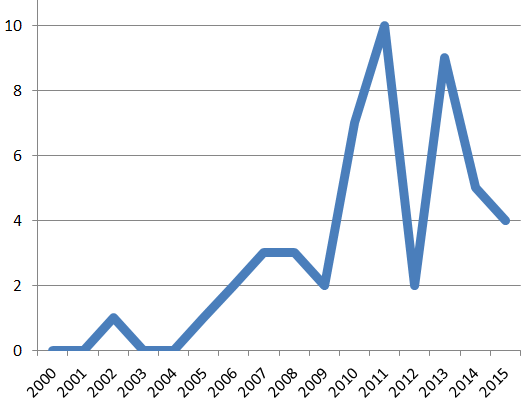
\includegraphics[scale=0.6]{PublicacionesAnuales.png}
  \end{center}
  \caption{Distribución de las publicaciones por años}
  \label{fig:PublicacionesAnuales}
\end{figure}

\subsection{Categorización del estudio}

Una vez revisados todos los artículos, se han extraído unas características o categorías comunes a la tipología de los trabajos. Todos los trabajos seleccionados hacen uso de algún tipo de software o metodología para evaluar algún tipo de competencia genérica. Sólo dos trabajos mencionan un enfoque como el que se propone en la introducción de este capítulo, es decir, aprovechando los registros de interacción de los estudiantes con el LMS como indicadores del desempeño de las competencias genéricas. Encontramos trabajos que se apoyan en la tecnología para el tratamiento o evaluación de las competencias, pero que terminan delegando parte de esta evaluación en el alumnado, ya sea mediante autoevaluación o evaluación entre iguales. Otros trabajos se basan en videojuegos o en las redes sociales para evaluar alguna competencia, mientras que otros desarrollan algún tipo de software o técnica. Finalmente hay algunos trabajos que simplemente detectan en su entorno la necesidad de la evaluación de las competencias de manera automática porque su forma de hacerlo les ocasiona una serie de problemas o desventajas con respecto a otro método que proponen o demandan. Además se han encontrado algunas revisiones sobre la literatura relacionadas que también serán tratadas aparte.  En la tabla \ref{tab:PublicacionesForum} se puede ver la distribución de las publicaciones. Algunos trabajos utilizan más de un método simultáneamente. %, apoyadas gráficamente en la figura  \ref{fig:PublicacionesForum}.

\begin{table}
  \begin{center}
  \begin{tabular}{| m{10cm} | c |}
    \hline
    CATEGORÍA & TRABAJOS\\
    \hline
    \hline 
    Peer and self-assessment & 18\\
    \hline
    Teacher assessment & 21\\
    \hline
    Questionaries & 16\\
    \hline
    Learning Analytics & 2\\
    \hline
  \end{tabular}
\end{center}
\caption{Distribución de publicaciones por tratamiento del problema}
\label{tab:PublicacionesForum}
\end{table} 

%\begin{figure}
%  \begin{center}
%    \includegraphics[scale=0.4]{cap3_pub_forum.png}
%  \end{center}
%  \caption{Distribución de publicaciones por tratamiento del problema}
%  \label{fig:PublicacionesForum}
%\end{figure}

En la figura \ref{fig:Burble} se muestra la clasificación de los trabajos según su ámbito y su tipo (lado izquierdo), y según su ámbito y su contribución (lado derecho). La evaluación de competencias genéricas mediante el uso de las nuevas tecnologías es un tema poco desarrollado. No sólo corroborado porque hay pocos trabajos, si no también a partir de esta figura. La mayoría de los trabajos son propuesta s(\emph{Proposal of solution}), experiencias (\emph{Experience papers}), validaciones (\emph{Validation research}) y evaluaciones de la investigación (\emph{Evaluation research}), mientras que trabajos de opinión(\emph{Opinion papers}) o filosóficos (\emph{Philosophical papers}), trabajos típicos de un tema de investigación de cierta madurez, casi no hay.

El tipo de contribución está más distribuído. Las contribuciones del tipo proceso (\emph{Process}) y modelo (\emph{Model}) son las que se dan con más frecuencia, la primera con cuestionarios (\emph{Questionnarie}), evaluación del profesores (\emph{Teacher assessment}) y autoevaluaciones o evaluaciones entre compañeros (\emph{Peer and self-assessment}), mientras que la segunda se da con más frecuencia con cuestionarios y evaluaciones del profesor. 

\pagestyle{empty}
\begin{landscape}
\begin{figure}[H]
  \begin{center}
    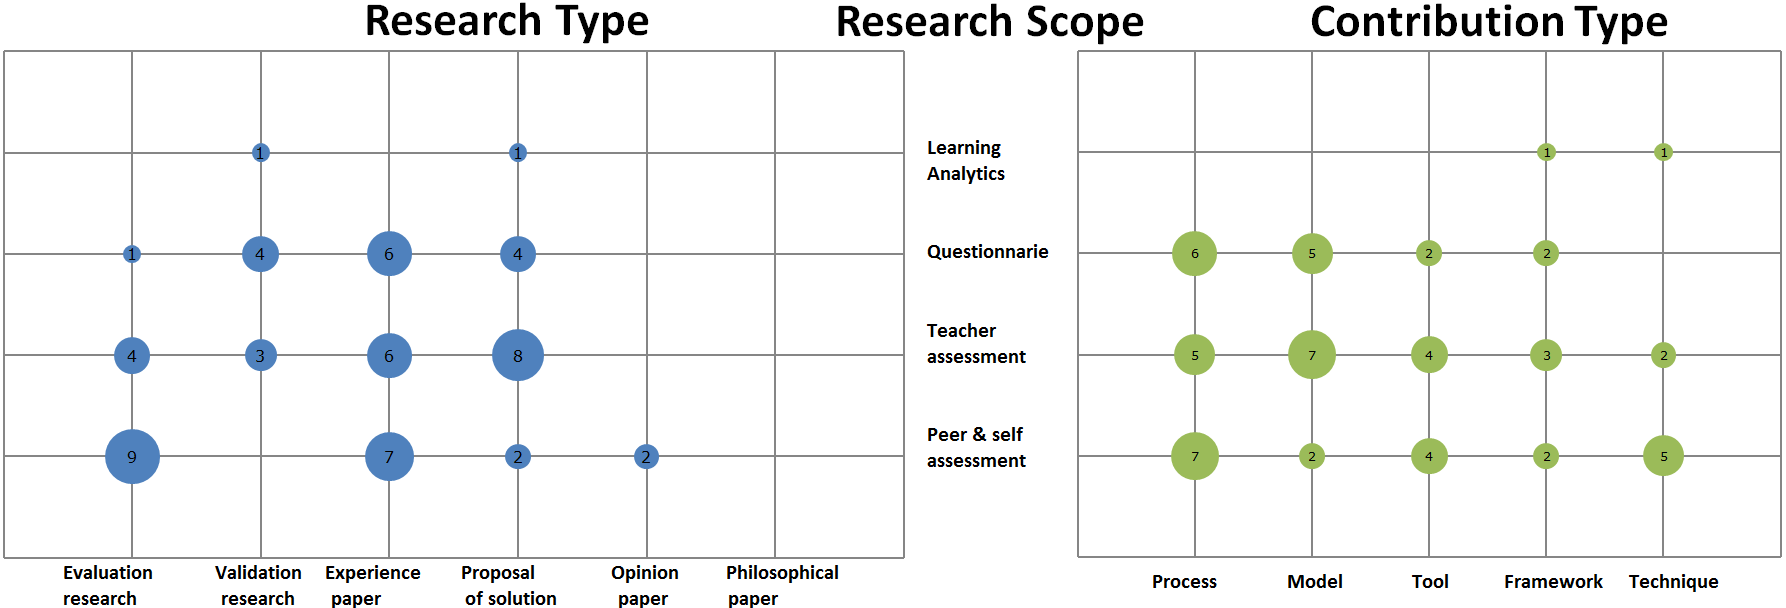
\includegraphics[scale=0.4]{Burbujas.png}
  \end{center}
  \caption{Ámbito de trabajos distribuidos según tipo de investigación y según tipo de contribución.}
  \label{fig:Burble}
\end{figure}
\end{landscape}
\pagestyle{fancy}

\subsection{Esquema de clasificación}

bla bla bla

\subsubsection{Peer and self-assessment}

La autoevaluación es un proceso en el que los estudiantes evaluan su propio trabajo, mientras que  en el proceso de evaluación entre iguales un estudiante evalúa el trabajo de otro u otros estudiantes. Esta práctica se emplea por un lado para ahorrar tiempo del profesorado, y por otro, para mejorar tanto el conocimiento en la materia del alumnado como sus habilidades metacognitivas. A menudo este tipo de evaluación se acompaña de algun tipo de rúbrica \cite{malehorn1994ten}.

Se han encontrado muchos trabajos en la literatura que utilizan este enfoque para evaluar competencias genéricas. De acuerdo a las preguntas de investigación de este trabajo únicamente se hanrecopilado aquellos trabajos que bajo este enfoque hagan uso de los ordenadores.

Se han encontrado varios trabajos que implementan una metodología de \emph{aprendizaje basado en problemas} (ABP o, del inglés, PBL, problem-based learning) para desarrollar competencias específicas y genéricas en sus estudiantes. En \cite{lasa2013problem} los profesores llevaron a cabo la evaluación del 90\% de las competencias utilizando la herramienta de rúbricas \emph{RubiStar}, mientras que los estudiantes mediante autoevaluación y evaluación entre iguales se encargaron del otro 10\%. En \cite{renau2010teaching} también se lleva a cabo una experiencia basada en una metodologia ABP para el desarrollo de la competencia en \emph{lengua extranjera} (inglés) en la que los estudiantes llevaban a cabo una autoevaluación de su nivel de adquisición de la competencia. En \cite{johnson2002encouraging} se muestran ejercicios para el desarrollo de competencias genéricas relacionados también con otra experiencia basada en una metodologia ABP y en unas presentaciones, siguiendo un enfoque de evaluaciones entre compañeros. En otro trabajo, vemos como los estudiantes después de haber realizado experiencias de videoconferencias en inglés, la competencia de \emph{inglés como lengua extranjera} junto con las competencias de \emph{trabajo en equipo} y \emph{comunicación oral} se evalúan en \cite{masip2013self} mediante auto y co-evaluación a través de Moodle.

El espíritu empresarial es considerado un factor fundamental para el desarrollo económico en todos los países del mundo \cite{DeXena2012educacion} y son muchos los trabajos que tratan de fomentar competencias genéricas relacionadas con las habilidades que un emprendedor ha de desempeñar. En \cite{chang2009international} se utiliza la herramienta Cycloid para el desarrollo de competencias en la gestión de proyectos y porteriormente se llevan a cabo autoevaluaciones de los propios estudiantes para valorar la adquisición de dichas competencias. En \cite{marquez2010have} se autoevalúan las competencias de \emph{iniciativa} y \emph{espíritu emprendedor}. También se autoevaluan competencias \emph{empresariales} en  \cite{achcaoucaou2014competence} mediante el uso de Tricuspoid. 

Un e-portfolio (del inglés \emph{electronic portfolio}, consiste en un conjunto de documentos, generalmente textos, archivos e imágenes, gestionados en un entorno web por un usuario. Se han recopilado trabajos donde los estudiantes trabajan con esta herramienta durante el curso y al final autoevalúan el desempeño de alguna competencia genérica. Por ejemplo, en \cite{arno2011promoting} se lleva a cabo una autoevaluación de la competencia del \emph{pensamiento crítico} tras haber trabajado en un e-portfolio. Mientras que en \emph{starcic2008sustaining} se utiliza también un e-portfolio para el desarrollo profesional de los estudiantes y se facilitan rubricas para la propia autoevaluación después de sus competencias genéricas.

En muchos trabajos la autoevaluación completa algún otro tipo de evaluación. En \cite{sevilla2012assessment} se utiliza plataforma online inGenio Tester para evaluar el nivel de adquisición de competencias en las modalidades de autoevaluación y evaluación por parte del profesor. En \cite{ficapal2015learning} se presenta un modelo que persigue el aprendizaje basado en equipos para la adquisición y evaluación de competencias genéricas en un contexto de e-learning. Los estudiantes trabajaban en grupo y evaluaban su desempeño en el \emph{trabajo en equipo} mediante una rúbrica. La calificación se completó con un cuestionario. En \cite{khamis2012measurement} también se trabajó y evaluó la competencia de \emph{trabajo en equipo}. Para ello los estudiates trabajaron en equipo y la evaluación tenía dos partes: por un lado los compañeros eran evaluados por otros compañeros (evaluación entre iguales) y por otro lado, también el profesor formaba parte de esta evaluación. En \cite{barbera2011assessment} se desarrollan y evalúan el desarrollo y desempeño de tres competencias genéricas en sus estudiantes: \emph{comunicación verbal}, \emph{comunicación escrita} y \emph{trabajo en equipo}. Este estudio propone una metodología basada en el modelo de tres niveles de evaluación de competencias utilizado por la Universidad de Deusto mediante diferentes herramientas utilizando tres tipos de evaluaciones: autoevaluación, evaluación entre iguales y evaluación del profesor.

Las herramientas 2.0 como wikis o blogs también se utilizan para medir el desempeño en competencias genéricas. En \cite{piedra2010measuring} se utilizan una serie de rúbricas para la autoevaluación de los estudiantes a partir de una serie de indicadores del desempeño de las competencias genéricas de la \emph{creatividad} y del \emph{trabajo colaborativo} a partir de su trabajo en herramientas de trabajo colaborativo. En \cite{mcloughlin2006beyond} se presentan una revisión de herramientas online para trabajar y evaluar competencas genéricas. Entre ellas también se mencionan herramientas colaborativas para la competencia del \emph{trabajo en equipo}.

Para la evaluación de la competencia de la capacidad \emph{autocrítica} se realizó una experiencia en \cite{pinto2011assessment}, dónde un conjunto de profesores de diferentes titulaciones establecieron actividades para los estudiantes. Estos estudiantes evaluaron su propio trabajo. Para medir el grado de competencia de los estudiantes se utilizó la diferencia de la nota entre la que recibieron los estudiantes por parte del profesor y la que ellos mismos se pusieron. En \cite{sin2007evaluating} también se realizó una experiencia donde tanto los propios estudiantes como los profesores evaluaban el desempeño de las competencias de la comunicación en contabilidad, tanto las \emph{habilidades para expresarse de manera escrita} como del \emph{pensamiento analítico}.

Aunque la autoevaluación y evaluación entre iguales son enfoques que quitan trabajo al docente, no todos son ventajas. Como se ha visto en algunos trabajos anteriores, este enfoque a menudo sólo se utiliza de manera complementaria a algún otro tipo de evaluación. Además, se puede dar el caso que la autoevaluación no se ajuste del todo a la realidad del desempeño del estudiante. Por ejemplo, en \cite{carreras2013promotion} hay notables diferencias entre las calificaciones que se auto-asignan los estudiantes en algunas competencias y las calificaciones que le asignaron los profesores en esas mismas competencias. En ese trabajo se promovió la adquisición de competencias genéricas desde un punto de vista interdisciplinar y se diseñaron herramientas especifícas para evaluar dichas habilidades. A la hora de evaluar, se realizaron tanto autoevaluaciones como evaluaciones del profesor. En esta experiencia se evaluaron cuatro competencias genéricas: \emph{capacidad de análisis},  \emph{habilidades de escritura}, \emph{responsabilidad} y \emph{capacidad de trabajo en equipo}. Cabe destacar discrepancias entre las calificaciones que se auto-asignan los estudiantes en las dos primeras competencias. En la \emph{capacidad de análisis} la discrepancia es de un 55,65\%, mientras que en las \emph{habilidades de escritura} de un 13,75\%.

\subsubsection{Teacher assessment}

En muchos casos la evaluación de competencias genéricas se realiza mediante un seguimiento continuo del trabajo del estudiante por parte del profesor. Este proceso es lo que se conoce como \emph{evaluación continua}. Esto permite ir introduciendo mejoras constantes en el proceso de aprendizaje, siendo éste el motivo por el que la evaluación continua se adopta como una estrategia de evaluación formativa más orientada al proceso de aprendizaje que a una valoración puntual. Actualmente, los expertos, influenciados por la \emph{Declaración de Bolonia}, consideran más apropiado desarrollar este tipo de sistemas de evaluación~\cite{garcia2005competencias}. 

En trabajos como los mostrados en \cite{martin2010new,prashar2010competence}, el profesorado sigue una metodología de evaluación continua para evaluar las competencias de \emph{trabajo en equipo} y \emph{comunicación oral y escrita}. Se establecen una serie de indicadores que les permiten monitorizar el progreso de los estudiantes. Una herramienta que se suele utilizar para hacer un seguimiento del trabajo de los estudiantes a lo largo del curso es el e-portfolio. En \cite{martin2013acquired,rodriguez2010portfolio,benlloch2007adapting} los profesores evalúan el desempeño de los estudiantes en las competencias de \emph{trabajo en equipo} y \emph{habilidades de comunicación} o \emph{solución de problemas}, entre otras. Para ello utilizan el e-portfolio, aunque en todos los casos combinan la evaluación del trabajo realizado por cada estudiante en el suyo junto con la calificaciones de otras actividades, exámenes y cuestionarios.

En \cite{yang2014fine} se define un modelo de itinerario de aprendizaje que soporta la evaluación de algunos conocimientos y competencias para describir el progreso de aprendizaje del estudiante. El modelo se define matemáticamente para poder formalmente definir las evaluaciones y para poder reutilizar las fórmulas. Aunque se reconoce las ventajas de un sistema que automatice este proceso, hasta el momento son los profesores los que evalúan a sus estudiantes en cada una de sus etapas. Además, muestran su reticencia a un sistema 100\% automático. Las competencias de \emph{comunicación} y \emph{escritura} se evalúan en este trabajo.

Uno de los problemas de la no automatización de los procesos de evaluación es la escalabilidad de algunos procesos de evaluación. En \cite{serrano2013hiperion} se diseña \emph{Hiperion}, una sistema de recomendación que ayuda a diseñar actividades adaptadas a cada estudiante para mejorar sus competencias. En el estudio de caso mostrado en este trabajo, los profesores evaluaban las competencias de los estudiantes manualmente y después aplicaban Hiperion. La principal desventaja de la herramienta es el tiempo que el profesor ha de dedicar para asignar los diferentes logros y el peso de cada nota para cada competencia en las actividades. En \cite{ward2011developing} se desarrollan una serie de módulos para Moodle para el desarrollo de competencias empresariales. Los alumnos realizan una serie de actividades para cada módulo y el profesor evalúa mediante conferencia via Skype si cada estudiante sabe lo que ha respondido. En \cite{lacuesta2009active} se utiliza una metodología ABP, dónde se realiza una evaluación individualizada de cada estudiante y de cada grupo de estudiantes. El autor considera que el esfuerzo necesario y carga de trabajo para cada profesor sólo es un poco mayor al habitual. En este trabajo se evaluan competencias como la \emph{capacidad critica}, \emph{trabajo en equipo}, \emph{planificación}, \emph{comunicación}, etc. Para minimizar el esfuerzo están las rúbricas, utilizadas en \cite{casan2015developing}, donde el docente se encarga mediante su uso de la evaluación en las habilidades de \emph{comunicación escrita} del alumnado.

\subsubsection{Questionnarie}

En \cite{lumsden2005assessment} se muestra la herramienta PQA (Personal Quality Assessment). Esta herramienta de evaluación contiene diversos test para la evaluación de la competencia genérica del \emph{razonamiento} y del {comportamiento ético} en el ámbito médico.

Trabajos: \cite{vizcarro2013assessment}, \cite{ruizacarate2013soft}, \cite{barbera2011design}, \cite{so2011mapping}, \cite{badcock2010developing}, \cite{aziz2007appraisal}, \cite{rashid2008engineering}, \cite{a2007outcome}, \cite{albergaria2011critical}, \cite{park2006moral}, \cite{andre2011formal}, \cite{martinez2014teamwork}, \cite{fernandez2011experience}.

\subsubsection{Learning Analytics}


% JUEGOS SERIOS BASADOS EN INDICADORES: ¿LOS SACO DE LA?

En \cite{guenaga2013serious} se utilizan los juegos serios para el desarrollo de las competencias de \emph{emprendimiento} y \emph{solución de problemas}. Se definieron una serie de indicadores para alcanzar  que se plasmaron en un juego que permite al estudiante conocer su nivel de adquisición en dichas competencias.

En \cite{bedek2011behavioral} también se utilizan los juegos serios para el desarrollo y evaluación de competencias genéricas. Se basa en un modelo donde para casa competencia se identifican subcompetencias más específicas, lo que facilita el proceso de definición de indicadores.

Trabajos: \cite{fidalgo:2015} and \cite{rayon2014web}

\section{Respuestas}


%\chapter{Trabajo en curso y futuro}

\section{Conclusiones}

\pagestyle{empty}
\begin{landscape}
\begin{center}
\begin{longtable}{| m{2.5cm} | m{9cm} | m{4cm} | m{2.5cm} | m{3.5cm} |}
    \hline
    REF & TÍTULO & TIPO DE INVESTIGACIÓN & TIPO DE CONTRIBUCIÓN & ÁMBITO DE LA INVESTIGACIÓN \\
    \hline
    \hline 
    \cite{yang2014fine} & A Fine-Grained Outcome-Based Learning Path Model & proposal of solution & model & Teacher assessment \\
    \hline
    \cite{rayon2014web} & A web platform for the assessment of competences in Mobile Learning Contexts & validation research & framework & Learning analytics \\
    \hline
    \cite{martin2013acquired} & Acquired Skills With The Implementation Of New Evaluation Methods At University Rey Juan Carlos & experience paper & model & Teacher assessment \\
    \hline
    \cite{lacuesta2009active} & Active learning through problem based learning methodology in engineering education & experience paper & process & Teacher assessment \\
    \hline
    \cite{benlloch2007adapting} & Adapting teaching and assessment strategies to enhance competence-based learning in the framework of the european convergence process & proposal of solution & process & Teacher assessment / Questionnarie \\
    \hline
    \cite{aziz2007appraisal} & Appraisal of Course Learning Outcomes using Rasch Measurement: A Case Study in Information Technology Education & proposal of solution & model & Questionnarie / Teacher assessment \\
    \hline
    \cite{sevilla2012assessment} & Assessment of competences in designing online preparatory materials for the Cambridge First Certificate in English examination & evaluation research & technique & Peer and self-assessment / Teacher assessment \\
    \hline
    \cite{lumsden2005assessment} & Assessment of personal qualities in relation to admission to medical school & evaluation research & framework & Questionnarie \\
    \hline
    \cite{vizcarro2013assessment} & Assessment of problem solving in computing studies & experience paper & process & Questionnarie \\
    \hline
    \cite{pinto2011assessment} & Assessment Of Self-Criticism Capacity Competence In Higher Education Students: Outcome Oriented Education & experience paper & process & Peer and self-assessment \\
    \hline
    \cite{barbera2011assessment} & Assessment Tools For The Evaluation Of Generic Skills Development In Students Of Business Management & proposal of solution & model & Teacher assessment \\
    \hline
    \cite{mcloughlin2006beyond} & Beyond marks and measurement: Developing dynamic and authentic forms of e-assessment & opinion paper & technique & Peer and self-assessment \\
    \hline
    \cite{achcaoucaou2014competence} & Competence Assessment in Higher Education: A Dynamic Approach & proposal of solution & tool & Peer and self-assessment \\
    \hline
    \cite{prashar2010competence} & Competence Based Teaching And Evaluation In The General Chemistry Course Of The University Rey Juan Carlos & experience paper & framework & Teacher assessment \\
    \hline
    \cite{strijbos2015criteria} & Criteria and standards of generic competences at bachelor degree level: A review study & evaluation research & process & Pending \\
    \hline
    \cite{albergaria2011critical} & Critical Thinking, Questioning and Creativity as Components of Intelligence & proposal of solution & process & Questionnarie \\
    \hline
    \cite{barbera2011design} & "Design And Results Of Collaborative Project-Based Learning In The Subject Commercial Management"" In Industrial Organization Engineering""" & experience paper & framework & Questionnarie \\
    \hline
    \cite{ward2011developing} & Developing entrepreneurial accounting and finance competency using the ELLEIEC Virtual Centre for Enterprise & experience paper & tool & Teacher assessment \\
    \hline
    \cite{badcock2010developing} & Developing generic skills through university study: a study of arts, science and engineering in Australia & experience paper & model & Questionnarie \\
    \hline
    \cite{casan2015developing} & Developing Writing Skills in The Classroom: A Corpus-based Analysis of Multi-Genre Structures & proposal of solution & model & Teacher assessment \\
    \hline
    \cite{ficapal2015learning} & e-Learning and Team-based Learning. Practical Experience in Virtual Teams & experience paper & framework & Peer and self-assessment / Questionnarie \\
    \hline
    \cite{johnson2002encouraging} & Encouraging generic skills in science courses & proposal of solution & process & Peer and self-assessment / Teacher assessment \\
    \hline
    \cite{rashid2008engineering} & Engineering Students Performance Evaluation of Generic Skills Measurement: ESPEGS Model & validation research & model & Questionnarie / Teacher assessment \\
    \hline
    \cite{rodriguez2010portfolio} & e-Portfolio: A tool to assess university students' skills & evaluation research & tool & Teacher assessment \\
    \hline
    \cite{sin2007evaluating} & Evaluating a method of integrating generic skills with accounting content based on a functional theory of meaning & evaluation research & process & Peer and self-assessment / Teacher assessment \\
    \hline
    \cite{andre2011formal} & Formal model for assigning human resources to teams in software projects & validation research & model & Questionnarie \\
    \hline
    \cite{bedek2011behavioral} & From Behavioral Indicators to Contextualized Competence Assessment & proposal of solution & framework & Teacher assessment \\
    \hline
    \cite{oliver2013graduate} & Graduate attributes as a focus for institution-wide curriculum renewal: innovations and challenges & opinion paper & model & Peer and self-assessment \\
    \hline
    \cite{marquez2010have} & Have Our Future Entrepreneurs An Ethical Commitment? & evaluation research & process & Peer and self-assessment \\
    \hline
    \cite{serrano2013hiperion} & Hiperion: A fuzzy approach for recommending educational activities based on the acquisition of competences & proposal of solution & tool & Teacher assessment \\
    \hline
    \cite{chang2009international} & International creative tension study of university students in South Korea and Finland & evaluation research & tool & Peer and self-assessment \\
    \hline
    \cite{} & Making Explicit and Reinforcing Horizontal Competences in an Electronic Engineering Degree & validation research & process & Teacher assessment \\
    \hline
    \cite{so2011mapping} & Mapping The Impact On Holistic Development: A Study Of The Relationship & proposal of solution & process & Questionnarie \\
    \hline
    \cite{khamis2012measurement} & Measurement of Students' Performance Level in a Group Project by using Peer Review and Lecturer Assessment & experience paper & technique & Peer and self-assessment / Teacher assessment \\
    \hline
    \cite{piedra2010measuring} & Measuring collaboration and creativity skills through rubrics: Experience from UTPL collaborative social networks course & evaluation research & process & Peer and self-assessment \\
    \hline
    \cite{park2006moral} & Moral competence and character strengths among adolescents: The development and validation of the Values in Action Inventory of Strengths for Youth & validation research & tool & Questionnarie \\
    \hline
    \cite{martin2010new} & New Methodologies In The Teaching And Evaluation Of The Competences “Teamwork” And “Oral And Written Communication” In The Civil Law Course Of The University Rey Juan Carlos & experience paper & framework & Teacher assessment \\
    \hline
    \cite{a2007outcome} & Outcome based education performance assessment: A computational model to measure electrical engineering subjects learning outcomes & evaluation research & model & Questionnarie /Teacher assessment \\
    \hline
    \cite{lasa2013problem} & Problem Based Learning Implementation In The Degree Of Human Nutrition And Dietetics & experience paper & technique & Peer and self-assessment / Teacher assessment \\
    \hline
    \cite{arno2011promoting} & Promoting reflection on science, technology, and society among engineering students through an EAP online learning environment & evaluation research & tool & Peer and self-assessment \\
    \hline
    \cite{masip2013self} & Self-video recording for the integration and assessment of generic competencies & experience paper & technique & Peer and self-assessment \\
    \hline
    \cite{guenaga2013serious} & Serious Games for the Development of Employment Oriented Competences & validation research & tool & Teacher assessment \\
    \hline
    \cite{ruizacarate2013soft} & Soft Skills: A Comparative Analysis Between Online and Classroom Teaching & experience paper & process & Questionnarie \\
    \hline
    \cite{starcic2008sustaining} & Sustaining Teacher's Professional Development and Training through Web-Based Communities of Practice & evaluation research & tool & Peer and self-assessment \\
    \hline
    \cite{renau2010teaching} & Teaching And Learning Through Projects Using The ICT: Practice Of The English Writing Through Business Documents & experience paper & process & Peer and self-assessment \\
    \hline
    \cite{martinez2014teamwork} & Teamwork competence and academic motivation in computer science engineering studies & validation research & process & Questionnarie \\
    \hline
    \cite{fernandez2011experience} & The experience of implementing a communication skills assessment in the first year course for undergraduate computing engineering students: A tool for further development of an international curriculum & experience paper & tool & Questionnarie \\
    \hline
    \cite{carreras2013promotion} & The promotion and assessment of generic skills from interdisciplinary teaching teams & experience paper & process & Peer and self-assessment / Teacher assessment \\
    \hline
    \cite{fidalgo:2015} & Using Learning Analytics to improve teamwork assessment & proposal of solution & technique & Learning analytics \\
    \hline
\caption{Distribución de publicaciones por tratamiento del problema}
\label{tab:ListadoTrabajos}
\end{longtable}
\end{center}
\end{landscape}

\pagestyle{fancy}


% ----------------------------------------------------------------------

	

%: ----------------------- overall methodology ------------------------
% introduction

% this file is called up by thesis.tex
% content in this file will be fed into the main document

%: ----------------------- introduction file header -----------------------
\begin{savequote}[50mm]
Historical methodology, as I see it, is a product of common sense applied to circumstances. 
\qauthor{Samuel E. Morison}
\end{savequote}


\chapter{Diseño y desarrollo de la metodología para la evaluación de competencias genéricas}
\label{cha:Overall methodology}

% the code below specifies where the figures are stored
\ifpdf
    \graphicspath{{3_overall_methodology/figures/PNG/}{3_overall_methodology/figures/PDF/}{3_overall_methodology/figures/}}
\else
    \graphicspath{{3_overall_methodology/figures/EPS/}{3_overall_methodology/figures/}}
\fi


%------------------------------------------------------------------------- 

\cite{turing1950computing}

Este capítulo presenta los requisitos, diseño y desarrollo de los sistemas empleados para guiar la evaluación de competencias genéricas: EvalCourse, AMW y EvalSim.

% Tengo que estudiar esta división. EvalCourse y EvalSim son DSLs para LMS y Mundos virtuales respectivamente. AMW es un sistema para escalar la evaluación del trabajo en Wikis mediante la peer y autoevaluación.

% Otra pata de la tesis era BISE. aplicado el DSL al organizational learning. Creo que las 3 patas son esas:
% LMS
% Mundos virtuales
% Organizational Learning

% AMW no es una pata como tal. ¿Se queda fuera por tanto?

\section{Requisitos}

\section{Diseño}

\section{Implementación}






% ----------------------------------------------------------------------


	
%: ----------------------- experiments and results ------------------------
% introduction

% this file is called up by thesis.tex
% content in this file will be fed into the main document

%: ----------------------- introduction file header -----------------------
\begin{savequote}[50mm]
The logic of validation allows us to move between the two limits of dogmatism and skepticism. 
\qauthor{Paul Ricoeur}
\end{savequote}


\chapter{Validation of the methodology}
\label{cha:Validation of the methodology}

% the code below specifies where the figures are stored
\ifpdf
    \graphicspath{{4_experiments_and_results/figures/PNG/}{4_experiments_and_results/figures/PDF/}{4_experiments_and_results/figures/}}
\else
    \graphicspath{{4_experiments_and_results/figures/EPS/}{4_experiments_and_results/figures/}}
\fi


%------------------------------------------------------------------------- 

\cite{turing1950computing}

Lorem ipsum dolor sit amet, consectetur adipiscing elit. Ut ultrices egestas nunc, venenatis rhoncus elit fermentum non. Pellentesque gravida nulla vitae ipsum lobortis ullamcorper. Ut adipiscing, tellus in egestas mattis, enim metus pretium erat, ac tempor dolor neque placerat nulla. Nullam nec ligula eu ipsum pharetra semper a in magna. Integer ut tortor quis nisi fringilla euismod eu ac ipsum. Pellentesque sodales consectetur erat eget rutrum. Proin ornare dolor ut arcu aliquet vestibulum. Pellentesque laoreet tincidunt sem eget semper.

Integer interdum mattis magna ullamcorper tristique. Nullam commodo nulla eget ipsum vulputate tincidunt auctor leo aliquet. Fusce euismod sagittis ante, eu vulputate eros dictum at. Cras non euismod nunc. Nullam velit diam, consectetur sed eleifend vitae, blandit at arcu. Maecenas ut urna nec turpis lobortis commodo. Aliquam aliquet turpis id massa viverra id sollicitudin est cursus. Sed a tortor non mauris cursus imperdiet.

Integer fermentum rutrum urna at vestibulum. Vivamus ullamcorper erat in sapien dignissim pellentesque. Integer convallis fringilla dictum. In bibendum lectus eu nulla pretium volutpat. Morbi hendrerit fringilla tortor, sed gravida neque lacinia a. In risus magna, hendrerit vitae cursus ac, vehicula at eros. Aenean quis ipsum sit amet leo vestibulum cursus.

Cras placerat mattis dui quis vehicula. Nulla sit amet metus nibh, at auctor enim. Quisque congue ultricies sapien in suscipit. Fusce vitae placerat ante. Praesent aliquet urna ac elit consequat nec mattis augue faucibus. Nunc et sapien vel felis mollis sodales. Aenean molestie nulla vestibulum nisi fringilla vel euismod dolor tristique. Aenean fermentum, dolor eget tincidunt faucibus, risus lorem feugiat elit, sagittis malesuada eros ligula in odio. Pellentesque ac libero lobortis justo bibendum laoreet. Cras egestas lorem eget ligula dignissim sollicitudin. Vestibulum sit amet augue ultrices erat faucibus vestibulum. Aenean tincidunt faucibus leo, nec auctor diam bibendum a. Sed varius, mauris in pellentesque scelerisque, nisl ligula viverra erat, in eleifend tellus enim ac magna. Pellentesque quis est risus. Cras mollis feugiat auctor. Proin ac eros vitae nulla gravida varius.

Morbi at augue sapien. Duis tempus quam vitae velit interdum ultricies. Vivamus laoreet lacinia elit sit amet vehicula. Ut congue diam ac magna hendrerit sed fermentum justo lacinia. Curabitur vel odio neque, quis consequat mi. Proin lobortis justo quis enim fermentum accumsan sagittis ipsum imperdiet. Proin sem felis, laoreet placerat egestas id, fringilla id mauris. Pellentesque a nisi sit amet leo consectetur gravida nec et dui. Curabitur quis hendrerit augue. Etiam sed dui nec tortor convallis fringilla. Proin tempor mattis diam nec egestas. Quisque condimentum elementum lacus ac porta. Vivamus congue, odio eu ullamcorper elementum, leo turpis tempus sem, at condimentum dolor quam eu nunc. Pellentesque eget risus ac velit aliquam sollicitudin sed et ipsum. 










% ----------------------------------------------------------------------

	
\section{Caso 1: Wikis}	
\section{Caso 2: Cursos virtuales}	
\section{Caso 3: EvalSim aplicado a mundos virtuales}	
	
%: ----------------------- conclusion ------------------------
% introduction

% this file is called up by thesis.tex
% content in this file will be fed into the main document

%: ----------------------- introduction file header -----------------------
\begin{savequote}[50mm]
Now this is not the end. It is not even the beginning of the end. But it is, perhaps, the end of the beginning. 
\qauthor{Winston Churchill}
\end{savequote}


\chapter{Conclusiones y trabajo futuro}
\label{cha:Conclusions}

% the code below specifies where the figures are stored
\ifpdf
    \graphicspath{{5_conclusion/figures/PNG/}{5_conclusion/figures/PDF/}{5_conclusion/figures/}}
\else
    \graphicspath{{5_conclusion/figures/EPS/}{5_conclusion/figures/}}
\fi


%------------------------------------------------------------------------- 

\cite{turing1950computing}

Lorem ipsum dolor sit amet, consectetur adipiscing elit. Ut ultrices egestas nunc, venenatis rhoncus elit fermentum non. Pellentesque gravida nulla vitae ipsum lobortis ullamcorper. Ut adipiscing, tellus in egestas mattis, enim metus pretium erat, ac tempor dolor neque placerat nulla. Nullam nec ligula eu ipsum pharetra semper a in magna. Integer ut tortor quis nisi fringilla euismod eu ac ipsum. Pellentesque sodales consectetur erat eget rutrum. Proin ornare dolor ut arcu aliquet vestibulum. Pellentesque laoreet tincidunt sem eget semper.

Integer interdum mattis magna ullamcorper tristique. Nullam commodo nulla eget ipsum vulputate tincidunt auctor leo aliquet. Fusce euismod sagittis ante, eu vulputate eros dictum at. Cras non euismod nunc. Nullam velit diam, consectetur sed eleifend vitae, blandit at arcu. Maecenas ut urna nec turpis lobortis commodo. Aliquam aliquet turpis id massa viverra id sollicitudin est cursus. Sed a tortor non mauris cursus imperdiet.

Integer fermentum rutrum urna at vestibulum. Vivamus ullamcorper erat in sapien dignissim pellentesque. Integer convallis fringilla dictum. In bibendum lectus eu nulla pretium volutpat. Morbi hendrerit fringilla tortor, sed gravida neque lacinia a. In risus magna, hendrerit vitae cursus ac, vehicula at eros. Aenean quis ipsum sit amet leo vestibulum cursus.

Cras placerat mattis dui quis vehicula. Nulla sit amet metus nibh, at auctor enim. Quisque congue ultricies sapien in suscipit. Fusce vitae placerat ante. Praesent aliquet urna ac elit consequat nec mattis augue faucibus. Nunc et sapien vel felis mollis sodales. Aenean molestie nulla vestibulum nisi fringilla vel euismod dolor tristique. Aenean fermentum, dolor eget tincidunt faucibus, risus lorem feugiat elit, sagittis malesuada eros ligula in odio. Pellentesque ac libero lobortis justo bibendum laoreet. Cras egestas lorem eget ligula dignissim sollicitudin. Vestibulum sit amet augue ultrices erat faucibus vestibulum. Aenean tincidunt faucibus leo, nec auctor diam bibendum a. Sed varius, mauris in pellentesque scelerisque, nisl ligula viverra erat, in eleifend tellus enim ac magna. Pellentesque quis est risus. Cras mollis feugiat auctor. Proin ac eros vitae nulla gravida varius.

Morbi at augue sapien. Duis tempus quam vitae velit interdum ultricies. Vivamus laoreet lacinia elit sit amet vehicula. Ut congue diam ac magna hendrerit sed fermentum justo lacinia. Curabitur vel odio neque, quis consequat mi. Proin lobortis justo quis enim fermentum accumsan sagittis ipsum imperdiet. Proin sem felis, laoreet placerat egestas id, fringilla id mauris. Pellentesque a nisi sit amet leo consectetur gravida nec et dui. Curabitur quis hendrerit augue. Etiam sed dui nec tortor convallis fringilla. Proin tempor mattis diam nec egestas. Quisque condimentum elementum lacus ac porta. Vivamus congue, odio eu ullamcorper elementum, leo turpis tempus sem, at condimentum dolor quam eu nunc. Pellentesque eget risus ac velit aliquam sollicitudin sed et ipsum. 

% ----------------------------------------------------------------------


	
	

% --------------------------------------------------------------
%:                  BACK MATTER: appendices, refs,..
% --------------------------------------------------------------

% the back matter: appendix and references close the thesis
\backmatter


%: ----------------------- appendix ------------------------

%\appendix


%: ----------------------- bibliography ------------------------



% The section below defines how references are listed and formatted
% The default below is 2 columns, small font, complete author names.
% Entries are also linked back to the page number in the text and to external URL if provided in the BibTex file.


% Original version:

% PhDbiblio-url2 = names small caps, title bold & hyperlinked, link to page 
%\begin{multicols}{2} % \begin{multicols}{ # columns}[ header text][ space]
%\begin{tiny} % tiny(5) < scriptsize(7) < footnotesize(8) < small (9)
%
%\bibliographystyle{Latex/Classes/PhDbiblio-url2} % Title is link if provided
%\renewcommand{\bibname}{References} % changes the header; default: Bibliography
%
%\bibliography{9_backmatter/references} % adjust this to fit your BibTex file
%
%\end{tiny}
%\end{multicols}



% Show all bibliography entries
%\nocite*



% If we want bibliography backreference, use unsrt first and the desidered one after

%\bibliographystyle{unsrt} % Defines the bibliography style

\bibliographystyle{alpha} % Defines the bibliography style

%\bibliographystyle{apa-good} % Defines the bibliography style
%\bibliographystyle{natbib} % Defines the bibliography style

%\bibliographystyle{plainurl}

%\renewcommand{\bibname}{References} % changes the header; default: Bibliography

%To include the references/works cited/bibliography in your Table of Contents, right before the bibliography command, use the command
%\addcontentsline{toc}{section}{References}
%

\bibliography{9_backmatter/references} % adjust this to fit your BibTex file

% --------------------------------------------------------------
% Various bibliography styles exit. Replace above style as desired.

% in-text refs: (1) (1; 2)
% ref list: alphabetical; author(s) in small caps; initials last name; page(s)
%\bibliographystyle{Latex/Classes/PhDbiblio-case} % title forced lower case
%\bibliographystyle{Latex/Classes/PhDbiblio-bold} % title as in bibtex but bold
%\bibliographystyle{Latex/Classes/PhDbiblio-url} % bold + www link if provided

%\bibliographystyle{Latex/Classes/jmb} % calls style file jmb.bst
% in-text refs: author (year) without brackets
% ref list: alphabetical; author(s) in normal font; last name, initials; page(s)

%\bibliographystyle{plainnat} % calls style file plainnat.bst
% in-text refs: author (year) without brackets
% (this works with package natbib)


% --------------------------------------------------------------


%: Declaration of originality

% this file is called up by thesis.tex
% content in this file will be fed into the main document

%: ----------------------- introduction file header -----------------------


% the code below specifies where the figures are stored
\ifpdf
    \graphicspath{{9_backmatter/figures/PNG/}{9_backmatter/figures/PDF/}{9_backmatter/figures/}}
\else
    \graphicspath{{9_backmatter/figures/EPS/}{9_backmatter/figures/}}
\fi

% Thesis statement of originality -------------------------------------

% Depending on the regulations of your faculty you may need a declaration like the one below. This specific one is from the medical faculty of the university of Dresden.

%\begin{declaration}        %this creates the heading for the declaration page

%Por la presente declaro que he realizado este trabajo sin la ayuda prohibido de terceros y sin hacer uso de las ayudas distintas de las especificadas; nociones tomadas en forma directa o indirecta de otras fuentes se han identificado como tal. Este trabajo no ha sido previamente presentado de manera idéntica o similar a cualquier mesa examinadora.

%The dissertation work was conducted from 20XX to \the\year \ under the supervision of
%Name Surname
%and 
%Name Surname
%at 
%the University Cádiz.

%\vspace{10mm}

% City
%Puerto Real,

% Signature figure

%\begin{flushright}
%\begin{figure}[htbp!]
%\end{figure}
%\includegraphics{signature}%
%\end{flushright}


%\end{declaration}



%-------------------------------------------------------------------------

\thispagestyle{empty}

\hfill
\vfill
\medskip

\begin{center}
\noindent
Este tesis doctoral fue finalizada en Jerez de la Frontera el 17 de junio de 2016
% Date
%\today 
\end{center}

\vfill
\medskip
\vspace{1cm}
\bigskip


%-------------------------------------------------------------------------

% Blank page
\clearpage
\thispagestyle{empty}

\hfill
\vfill
\medskip

\begin{center}
\textit{Esta página se ha dejado en blanco intencionadamente.}
\end{center}

\vfill
\medskip
\vspace{1cm}
\bigskip


% ----------------------------------------------------------------------






\end{document}
